\documentclass{article}
\usepackage{indentfirst}
\usepackage[T1]{fontenc}
\usepackage{graphicx}
\usepackage{booktabs}
\usepackage{array}
\usepackage{tabularx}
\usepackage{amsmath}
\usepackage{float}
\usepackage{caption}
\graphicspath{{Imagens/Diagramas/teoricas/}{../Imagens/Diagramas/teoricas/}}
\renewcommand{\figurename}{Figura}
\renewcommand{\tablename}{Tabela}
\captionsetup{
  justification=raggedright,
  singlelinecheck=false,
  labelsep=endash,
  font=small,
  labelfont=bf,
  skip=6pt
}
\captionsetup[figure]{position=above}
\captionsetup[table]{position=above}
\newfloat{quadro}{htbp}{loq}
\floatname{quadro}{Quadro}
\captionsetup[quadro]{position=above}
\newcommand{\fonteelemento}[1]{%
  \par\smallskip
  {\footnotesize\raggedright Fonte: #1.\par}%
}

\begin{document}

\section{Fundamenta\c{c}\~ao Te\'orica}


\subsection{Sistemas embarcados vest\'iveis}


Sistemas embarcados vest\'iveis s\~ao dispositivos computacionais concebidos para uso junto ao corpo e para opera\c{c}\~ao durante as atividades do usu\'ario. Eles combinam processamento, sensores, comunica\c{c}\~ao, interface e alimenta\c{c}\~ao em um volume limitado, o que imp\~oe restri\c{c}\~oes simult\^aneas de \'area, mem\'oria, capacidade computacional e energia. Diferentemente de instrumentos de bancada, o posicionamento do dispositivo e os movimentos do usu\'ario tamb\'em passam a integrar as condi\c{c}\~oes de medi\c{c}\~ao.


Uma plataforma vest\'ivel multissensor re\'une fun\c{c}\~oes com requisitos distintos. A interface gr\'afica demanda resposta percept\'ivel ao usu\'ario e transfer\^encias frequentes para o display; sensores podem exigir per\'iodos de aquisi\c{c}\~ao, tempos de convers\~ao e tratamentos de dados diferentes; servi\c{c}os compartilhados coordenam barramentos, mem\'oria e armazenamento. A concorr\^encia entre essas atividades precisa ser organizada sem perder de vista a capacidade limitada da plataforma.


A proximidade com o corpo favorece a aquisi\c{c}\~ao cont\'inua ou recorrente de sinais fisiol\'ogicos e de movimento, mas n\~ao elimina as limita\c{c}\~oes dos m\'etodos empregados. Contato vari\'avel, movimento, luz externa, posi\c{c}\~ao no punho e diferen\c{c}as entre usu\'arios podem alterar as medi\c{c}\~oes. Por isso, a disponibilidade de um sensor em um dispositivo vest\'ivel n\~ao \'e suficiente para atribuir validade cl\'inica aos valores produzidos, que depende de procedimento de valida\c{c}\~ao compat\'ivel com a finalidade declarada (SENEVIRATNE et al., 2017).


\subsubsection{Plataforma computacional embarcada}


A sele\c{c}\~ao de uma plataforma computacional para um vest\'ivel envolve compromissos entre dimens\~oes, consumo, interfaces dispon\'iveis, mem\'oria, capacidade de processamento, ecossistema de desenvolvimento e possibilidade de integrar os perif\'ericos previstos. Esses crit\'erios devem ser relacionados \`a carga da aplica\c{c}\~ao e \`as interfaces necess\'arias; a simples disponibilidade de maior frequ\^encia de clock ou conectividade n\~ao demonstra adequa\c{c}\~ao ao sistema.


O ESP32-C6 integra um processador principal RISC-V de 32 bits, com frequ\^encia de at\'e 160 MHz, 512 KiB de SRAM de alto desempenho e 16 KiB de SRAM de baixo consumo, al\'em de interfaces como I$^2$C, SPI, RMT, USB Serial/JTAG e conversor anal\'ogico-digital SAR de 12 bits (ESPRESSIF SYSTEMS, 2025a). Embora o circuito tamb\'em contenha um processador de baixo consumo, a configura\c{c}\~ao usual do FreeRTOS para a aplica\c{c}\~ao no processador principal \'e de n\'ucleo \'unico. Assim, tarefas concorrentes compartilham o mesmo tempo de CPU e n\~ao executam em paralelo nesse n\'ucleo.


O conjunto de instru\c{c}\~oes anunciado para o processador principal inclui extens\~oes inteiras, de multiplica\c{c}\~ao e divis\~ao, at\^omicas e comprimidas, mas n\~ao implementa as extens\~oes RISC-V de ponto flutuante de precis\~ao simples ou dupla (ESPRESSIF SYSTEMS, 2025b). Opera\c{c}\~oes em ponto flutuante permanecem dispon\'iveis pela linguagem e pela cadeia de compila\c{c}\~ao, por\'em podem recorrer a rotinas de software. Essa caracter\'istica recomenda avaliar a necessidade e a frequ\^encia dessas opera\c{c}\~oes, sem permitir inferir um custo quantitativo sem medi\c{c}\~ao.


A XIAO ESP32-C6 exp\~oe o circuito em uma placa de 21~mm por 17,8~mm, com USB, gerenciamento para bateria, 4 MiB de \emph{flash} e um conjunto reduzido de pinos (SEEED STUDIO, 2024). Essa combina\c{c}\~ao favorece um prot\'otipo compacto e o uso do ESP-IDF, mas tamb\'em imp\~oe limites: mem\'oria e pinos permanecem finitos, perif\'ericos podem ser compartilhados e a capacidade de processamento precisa atender simultaneamente \`a interface gr\'afica e aos sensores. Plataformas com mais pinos, mem\'oria externa ou mais n\'ucleos podem ser prefer\'iveis para outras cargas; a escolha \'e uma decis\~ao de engenharia situada, e n\~ao uma superioridade universal.


\subsection{Arquitetura modular de software}


Uma arquitetura de software descreve a organiza\c{c}\~ao de um sistema em elementos, as rela\c{c}\~oes entre eles e as decis\~oes que condicionam seu comportamento e sua evolu\c{c}\~ao. No caso de sistemas embarcados, essa organiza\c{c}\~ao precisa considerar n\~ao apenas a distribui\c{c}\~ao das fun\c{c}\~oes no c\'odigo, mas tamb\'em as depend\^encias de hardware, os servi\c{c}os compartilhados e as formas de comunica\c{c}\~ao entre partes executadas concorrentemente. A decomposi\c{c}\~ao em m\'odulos procura limitar o conhecimento que cada parte precisa manter sobre as demais.


Parnas (1972) prop\~oe que a divis\~ao de um sistema seja orientada pelas decis\~oes de projeto suscet\'iveis a mudan\c{c}a. Cada m\'odulo deve ocultar dos outros uma decis\~ao, representa\c{c}\~ao ou mecanismo que possa variar, expondo somente o necess\'ario para sua utiliza\c{c}\~ao. Esse crit\'erio difere de uma separa\c{c}\~ao baseada apenas na sequ\^encia de etapas do processamento: arquivos distintos ou fun\c{c}\~oes agrupadas por conveni\^encia n\~ao constituem, por si s\'os, uma arquitetura modular.


\subsubsection{Modularidade, coes\~ao e acoplamento}


A coes\~ao expressa o grau em que os elementos internos de um m\'odulo contribuem para uma responsabilidade bem definida. Um m\'odulo coeso re\'une dados e opera\c{c}\~oes relacionados ao mesmo prop\'osito, o que facilita sua compreens\~ao e reduz a necessidade de coordenar altera\c{c}\~oes internas sem rela\c{c}\~ao entre si. O acoplamento, por sua vez, caracteriza as depend\^encias entre m\'odulos, como o compartilhamento de dados, o conhecimento de representa\c{c}\~oes internas ou a depend\^encia de uma sequ\^encia particular de chamadas. No projeto estruturado, busca-se elevar a coes\~ao e reduzir o acoplamento para limitar a propaga\c{c}\~ao de altera\c{c}\~oes pelo sistema (STEVENS; MYERS; CONSTANTINE, 1974).


Baixo acoplamento n\~ao significa aus\^encia de intera\c{c}\~ao. Os m\'odulos precisam cooperar para que o sistema realize suas fun\c{c}\~oes, mas essa coopera\c{c}\~ao pode ocorrer por rela\c{c}\~oes expl\'icitas e restritas. Quando um m\'odulo depende apenas de uma interface est\'avel, altera\c{c}\~oes em sua implementa\c{c}\~ao interna tendem a permanecer localizadas. Em sentido oposto, o acesso direto ao estado interno, a duplica\c{c}\~ao de conhecimento e as depend\^encias impl\'icitas aumentam a quantidade de partes que precisam ser examinadas ou modificadas em conjunto.


Em plataformas embarcadas, o acoplamento tamb\'em pode decorrer do compartilhamento de recursos f\'isicos. Dois m\'odulos logicamente separados continuam relacionados se utilizam o mesmo barramento, perif\'erico ou regi\~ao de mem\'oria. A arquitetura deve tornar essa depend\^encia vis\'ivel e atribuir a um servi\c{c}o ou mecanismo definido a responsabilidade de coorden\'a-la. A separa\c{c}\~ao do c\'odigo n\~ao elimina conflitos de acesso ao hardware.


\subsubsection{Interfaces e contratos}


A interface de um m\'odulo estabelece os elementos pelos quais ele pode ser utilizado, enquanto oculta os detalhes que n\~ao devem ser conhecidos externamente. Ela pode especificar opera\c{c}\~oes dispon\'iveis, tipos de dados, estados poss\'iveis, condi\c{c}\~oes de chamada e formas de comunicar sucesso ou falha. Para preservar o isolamento, uma interface deve oferecer informa\c{c}\~ao suficiente ao uso correto do m\'odulo sem expor decis\~oes internas que possam mudar (PARNAS, 1972).


O conceito de contrato acrescenta \`as assinaturas das opera\c{c}\~oes as obriga\c{c}\~oes assumidas pelas partes envolvidas. Em sua formula\c{c}\~ao cl\'assica, um contrato explicita pr\'e-condi\c{c}\~oes que o chamador deve satisfazer, p\'os-condi\c{c}\~oes garantidas pela opera\c{c}\~ao e invariantes que permanecem v\'alidas durante o ciclo de vida do componente (MEYER, 1992). Em firmware escrito em C, um contrato pode ser expresso por tipos, valores de retorno, documenta\c{c}\~ao, conven\c{c}\~oes de estado e verifica\c{c}\~oes executadas pelo c\'odigo, mesmo quando n\~ao h\'a suporte nativo da linguagem para contratos formais.


Um contrato uniforme permite que o n\'ucleo trate m\'odulos distintos por um mesmo conjunto de expectativas. Isso n\~ao obriga todos os m\'odulos a possu\'irem implementa\c{c}\~oes ou meios de transporte id\^enticos. Diferen\c{c}as de hardware podem permanecer encapsuladas, desde que as opera\c{c}\~oes necess\'arias \`a integra\c{c}\~ao e o comportamento observ\'avel diante de sucesso ou falha estejam definidos. A Figura~\ref{fig:contrato-modular} sintetiza essa rela\c{c}\~ao entre o contrato p\'ublico, o estado interno dos m\'odulos e os servi\c{c}os compartilhados.


\begin{figure}[H]
\centering
\caption{Contrato uniforme e detalhes encapsulados em m\'odulos conceituais}
\label{fig:contrato-modular}
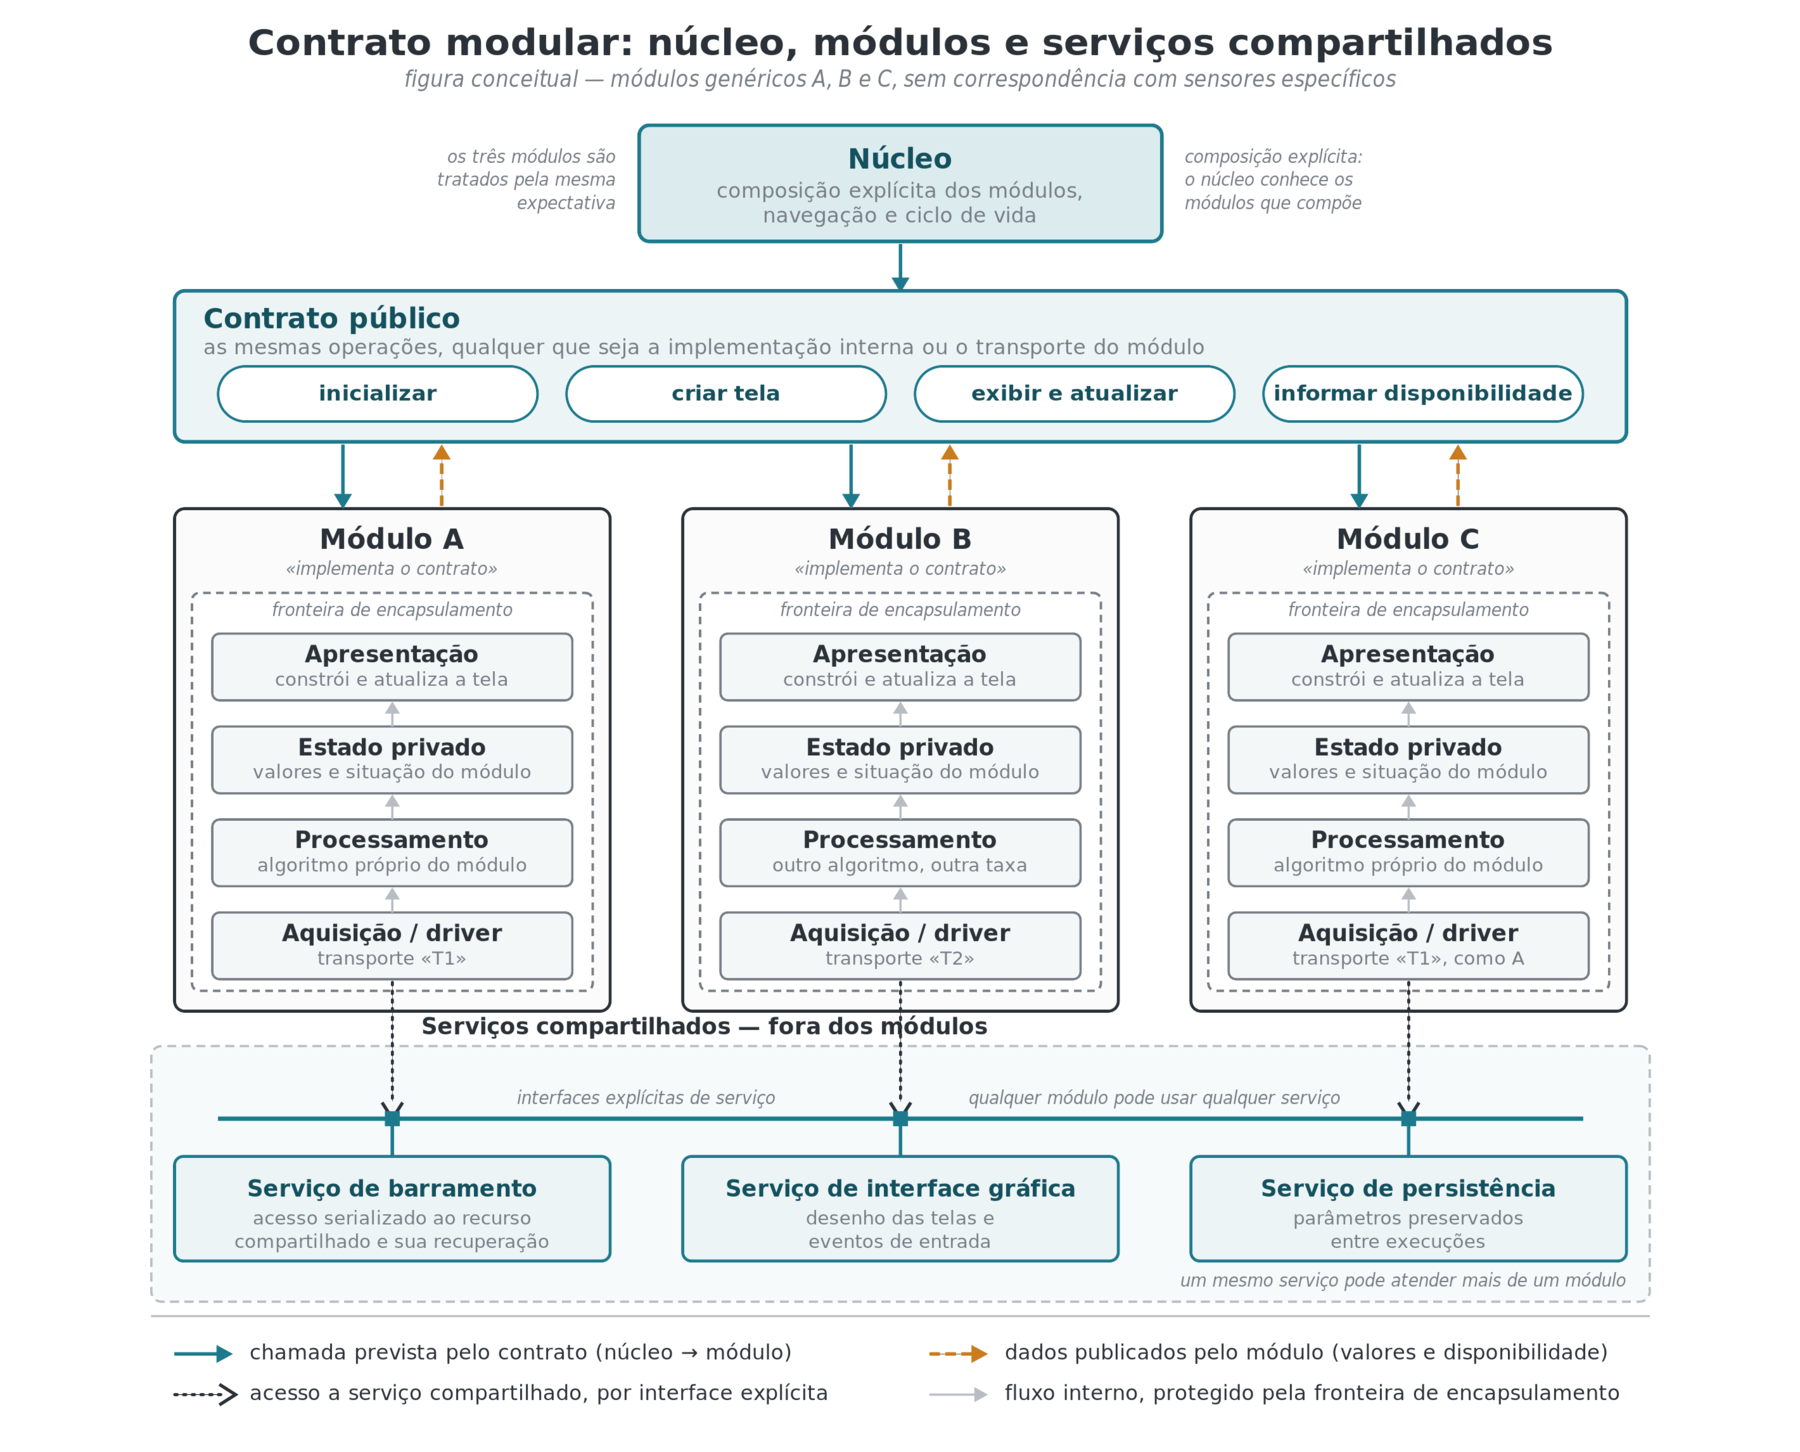
\includegraphics[width=0.96\textwidth]{contrato_modular.png}
\begin{minipage}{0.96\textwidth}
\fonteelemento{Elaborado pelo autor com base em Parnas (1972) e Meyer (1992)}
\end{minipage}
\end{figure}


O ciclo de vida de um m\'odulo pode compreender inicializa\c{c}\~ao, ativa\c{c}\~ao, opera\c{c}\~ao, desativa\c{c}\~ao e libera\c{c}\~ao de recursos. O contrato precisa distinguir um m\'odulo ainda n\~ao inicializado, dispon\'ivel, temporariamente indispon\'ivel ou em falha, de modo que chamadas fora do estado permitido possam ser rejeitadas de forma previs\'ivel. A inicializa\c{c}\~ao n\~ao fatal \'e uma pol\'itica arquitetural em que a indisponibilidade de uma fun\c{c}\~ao opcional \'e registrada e isolada, permitindo prosseguir com fun\c{c}\~oes sem depend\^encia daquele recurso.


\subsubsection{Separa\c{c}\~ao de responsabilidades}


Em firmware, uma decomposi\c{c}\~ao recorrente separa a adapta\c{c}\~ao ao hardware, o driver do dispositivo, o processamento do sinal, a tarefa de coordena\c{c}\~ao e a apresenta\c{c}\~ao. A camada de abstra\c{c}\~ao de hardware (Hardware Abstraction Layer --- HAL) representa capacidades do perif\'erico do microcontrolador; o driver traduz registradores e transa\c{c}\~oes do componente; o processamento transforma amostras em grandezas ou eventos; a tarefa define quando adquirir e publicar; e a apresenta\c{c}\~ao transforma o estado em elementos da interface.


Essa separa\c{c}\~ao reduz a propaga\c{c}\~ao de detalhes, mas n\~ao cria independ\^encia absoluta. Um algoritmo continua condicionado pela taxa de amostragem e pela faixa configuradas no hardware, e uma tela continua condicionada \`a disponibilidade e \`a validade dos dados. Em sistemas restritos, interfaces adicionais, c\'opias de dados e estados intermedi\'arios tamb\'em consomem mem\'oria e tempo. A abstra\c{c}\~ao deve preservar depend\^encias relevantes e ocultar apenas as decis\~oes que n\~ao precisam atravessar a fronteira do m\'odulo.


\subsubsection{Extensibilidade}


Extensibilidade \'e a capacidade de incorporar novas fun\c{c}\~oes ou ampliar fun\c{c}\~oes existentes com impacto controlado sobre a arquitetura. Ela n\~ao pode ser inferida apenas da exist\^encia de diret\'orios ou fun\c{c}\~oes separados. Sua avalia\c{c}\~ao requer um cen\'ario de mudan\c{c}a que identifique o est\'imulo, a parte modificada, as condi\c{c}\~oes da altera\c{c}\~ao e uma medida de resposta, como n\'umero de m\'odulos afetados, interfaces modificadas ou esfor\c{c}o necess\'ario (BASS; CLEMENTS; KAZMAN, 2021).


A extensibilidade depende das decis\~oes tomadas antecipadamente sobre pontos de varia\c{c}\~ao. Interfaces est\'aveis, responsabilidades localizadas e servi\c{c}os comuns reduzem a necessidade de repetir c\'odigo ou alterar o n\'ucleo a cada inclus\~ao. Entretanto, mecanismos gen\'ericos tamb\'em possuem custo de mem\'oria, processamento e complexidade. Em sistemas com recursos restritos, a arquitetura deve oferecer os pontos de extens\~ao necess\'arios ao problema sem introduzir abstra\c{c}\~oes cujo custo n\~ao seja justificado.


A demonstra\c{c}\~ao de extensibilidade deve observar uma modifica\c{c}\~ao concreta. A adi\c{c}\~ao de um novo m\'odulo, por exemplo, permite registrar quais arquivos e interfaces precisaram mudar e se m\'odulos existentes permaneceram inalterados. Esse procedimento produz evid\^encia mais direta do que a classifica\c{c}\~ao da arquitetura com base apenas em sua estrutura declarada.


\subsubsection{Toler\^ancia a falhas e continuidade das fun\c{c}\~oes independentes}


Na terminologia de dependabilidade, uma falha interna pode produzir um estado incorreto e, caso esse estado alcance a interface do sistema, resultar na interrup\c{c}\~ao ou na presta\c{c}\~ao incorreta de um servi\c{c}o. A toler\^ancia a falhas compreende os meios empregados para evitar que a presen\c{c}a de uma falha provoque a falha do servi\c{c}o oferecido (AVIZIENIS et al., 2004). Essa propriedade n\~ao equivale \`a impossibilidade de falhas nem garante, isoladamente, confiabilidade absoluta.


Em uma plataforma composta por fun\c{c}\~oes independentes, a falha ou aus\^encia de um sensor n\~ao precisa impedir a inicializa\c{c}\~ao dos demais m\'odulos. Para isso, a arquitetura deve conter o erro no subsistema afetado, comunicar sua indisponibilidade e preservar os servi\c{c}os que n\~ao dependem dele. A continuidade obtida est\'a limitada pelas depend\^encias reais: a falha de um recurso compartilhado pode afetar v\'arios m\'odulos e exige mecanismos espec\'ificos de coordena\c{c}\~ao, detec\c{c}\~ao e recupera\c{c}\~ao.


Esse comportamento deve ser avaliado pela introdu\c{c}\~ao controlada de falhas e pela observa\c{c}\~ao dos servi\c{c}os preservados. Ensaios com sensores ausentes, erros de comunica\c{c}\~ao e recupera\c{c}\~ao de recursos compartilhados permitem distinguir uma decis\~ao arquitetural implementada de uma propriedade efetivamente demonstrada.


\subsection{Sistemas operacionais de tempo real}


Um sistema operacional de tempo real (Real-Time Operating System --- RTOS) organiza a execu\c{c}\~ao de atividades concorrentes de acordo com requisitos temporais. Seu objetivo n\~ao \'e apenas executar opera\c{c}\~oes rapidamente, mas oferecer comportamento temporal suficientemente previs\'ivel para que eventos sejam tratados dentro dos limites definidos pela aplica\c{c}\~ao. Esses limites podem assumir a forma de per\'iodos de ativa\c{c}\~ao, prazos, lat\^encias m\'aximas ou tempos de resposta.


Em um sistema embarcado multissensor, o uso de um sistema operacional de tempo real permite representar aquisi\c{c}\~oes, processamento e interface como tarefas separadas. Essa decomposi\c{c}\~ao facilita a atribui\c{c}\~ao de per\'iodos e prioridades, mas n\~ao garante por si s\'o que os requisitos temporais sejam atendidos. O tempo de execu\c{c}\~ao das tarefas, as rela\c{c}\~oes de preced\^encia, o compartilhamento de recursos e os intervalos em que interrup\c{c}\~oes ou regi\~oes cr\'iticas impedem o escalonamento tamb\'em afetam o comportamento do sistema.


\subsubsection{Tarefas e escalonamento}


Uma tarefa representa um fluxo de execu\c{c}\~ao com contexto e pilha pr\'oprios. Durante sua exist\^encia, ela transita entre estados controlados pelo n\'ucleo: pode estar em execu\c{c}\~ao, pronta para executar, bloqueada \`a espera de tempo ou evento, ou suspensa explicitamente. Uma tarefa bloqueada n\~ao disputa o processador at\'e que sua condi\c{c}\~ao de desbloqueio seja satisfeita, o que permite aguardar per\'iodos, filas, notifica\c{c}\~oes ou recursos sem executar espera ocupada (FREERTOS, 2026a).


Em um escalonador preemptivo baseado em prioridades, a tarefa pronta de maior prioridade recebe o processador. Quando uma tarefa de prioridade superior se torna pronta, ela pode interromper a execu\c{c}\~ao de uma tarefa menos priorit\'aria. Tarefas de mesma prioridade podem compartilhar o processador por altern\^ancia temporal quando essa op\c{c}\~ao est\'a habilitada. A escolha das prioridades deve refletir requisitos de resposta e depend\^encias, pois atribuir prioridade elevada a uma atividade que executa continuamente pode impedir o progresso das demais.


O escalonamento de tarefas peri\'odicas \'e um problema cl\'assico de sistemas de tempo real. Liu e Layland (1973) demonstraram condi\c{c}\~oes de escalonabilidade para conjuntos de tarefas peri\'odicas independentes sob algoritmos de prioridade fixa e din\^amica. As hip\'oteses desses modelos, como independ\^encia entre tarefas e conhecimento de seus piores tempos de execu\c{c}\~ao, n\~ao s\~ao automaticamente satisfeitas em um firmware que compartilha barramentos e mutexes. Por isso, prioridades e per\'iodos precisam ser analisados em conjunto com os bloqueios introduzidos pela sincroniza\c{c}\~ao.


Em muitos sistemas operacionais de tempo real, um temporizador gera interrup\c{c}\~oes peri\'odicas denominadas \emph{ticks}. A cada ocorr\^encia, o n\'ucleo atualiza sua refer\^encia de tempo, verifica atrasos e limites de espera e pode liberar tarefas bloqueadas. A frequ\^encia do \emph{tick} determina a resolu\c{c}\~ao temporal dessas opera\c{c}\~oes: uma frequ\^encia mais alta oferece granularidade mais fina, mas aumenta a quantidade de interrup\c{c}\~oes executadas pelo n\'ucleo. Uma frequ\^encia mais baixa reduz essa sobrecarga, por\'em limita a resolu\c{c}\~ao dos atrasos expressos em m\'ultiplos de \emph{ticks}. Para tarefas peri\'odicas, atrasos relativos sucessivos podem acumular varia\c{c}\~ao de fase; mecanismos que utilizam como refer\^encia o instante de libera\c{c}\~ao anterior permitem manter um per\'iodo mais regular. Essa diferen\c{c}a temporal \'e representada na Figura~\ref{fig:tick-atrasos}.


\begin{figure}[H]
\centering
\caption{Diferen\c{c}a conceitual entre atrasos relativos e refer\^encia temporal peri\'odica}
\label{fig:tick-atrasos}
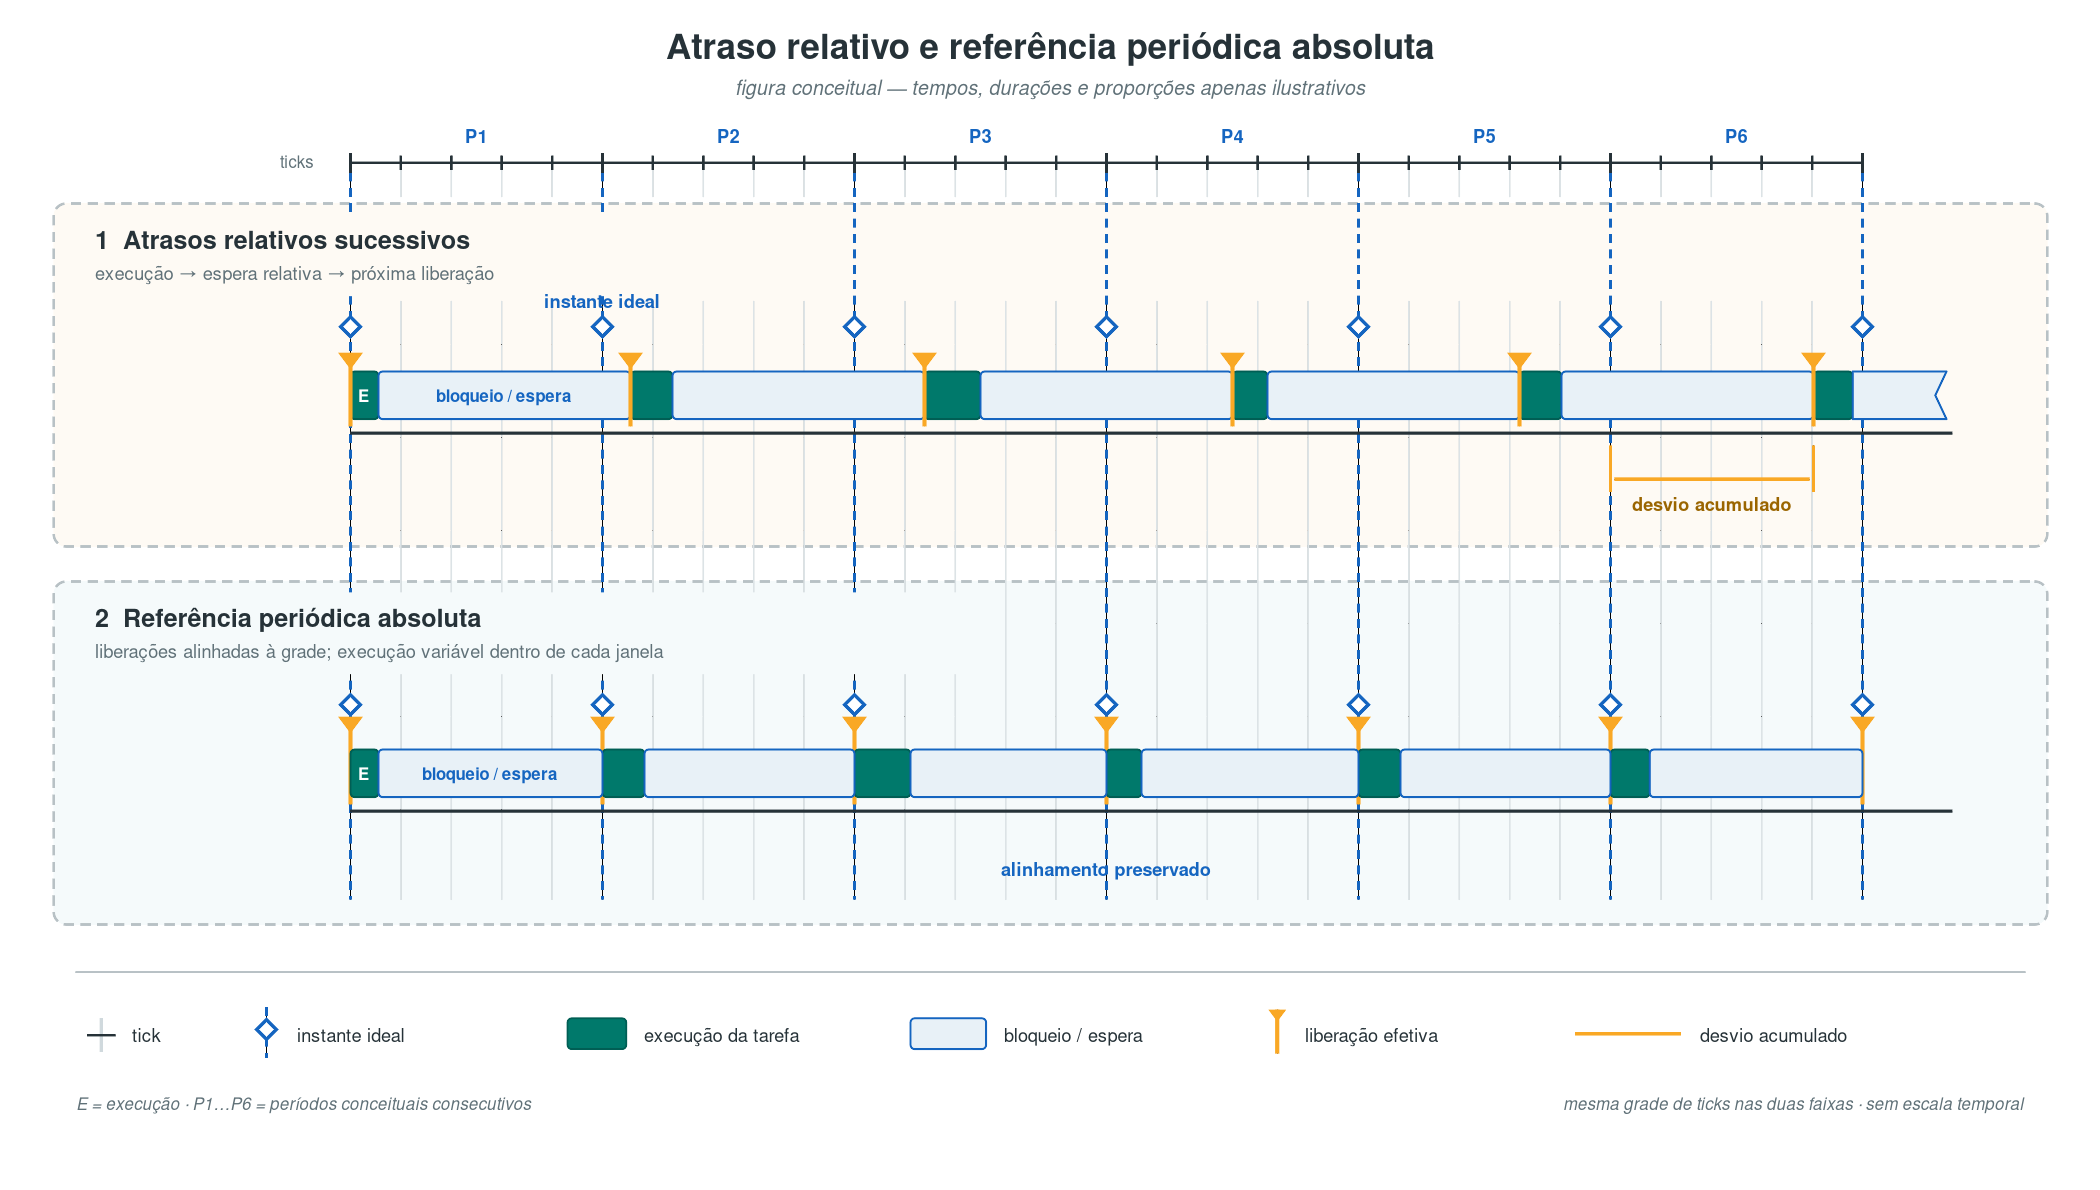
\includegraphics[width=0.94\textwidth]{tick_atrasos.png}
\fonteelemento{Elaborado pelo autor com base na documenta\c{c}\~ao do FreeRTOS (2026a)}
\end{figure}


\subsubsection{Sincroniza\c{c}\~ao e exclus\~ao m\'utua}


Tarefas concorrentes podem acessar dados ou recursos cuja utiliza\c{c}\~ao precisa ser coordenada. Sem sincroniza\c{c}\~ao, o resultado pode depender da ordem das opera\c{c}\~oes, produzindo condi\c{c}\~oes de corrida, estados parcialmente atualizados ou transa\c{c}\~oes sobrepostas. A necessidade de prote\c{c}\~ao depende tanto da atomicidade oferecida pelo processador quanto da sequ\^encia l\'ogica que deve permanecer indivis\'ivel.


A exclus\~ao m\'utua permite que somente uma tarefa por vez execute uma regi\~ao associada a um recurso compartilhado. O objeto de exclus\~ao m\'utua (mutex) possui rela\c{c}\~ao de propriedade: a tarefa que o obt\'em deve liber\'a-lo depois de concluir o acesso protegido. Essa caracter\'istica o diferencia de mecanismos usados apenas para sinaliza\c{c}\~ao de eventos. No FreeRTOS, mutexes incluem heran\c{c}a de prioridade, enquanto sem\'aforos bin\'arios n\~ao oferecem esse mecanismo (FREERTOS, 2026b).


O tempo durante o qual um mutex permanece retido afeta a lat\^encia das tarefas concorrentes. A regi\~ao protegida deve conter somente as opera\c{c}\~oes que precisam ser serializadas, sem atrasos deliberados ou processamento alheio ao recurso. Quando uma opera\c{c}\~ao de entrada e sa\'ida requer v\'arias etapas para preservar a integridade de uma transa\c{c}\~ao, liberar a prote\c{c}\~ao entre essas etapas pode permitir interfer\^encia de outra tarefa, ainda que reduza aparentemente o tempo de bloqueio.


O uso de v\'arios recursos protegidos tamb\'em pode criar espera circular. Se duas tarefas obt\^em mutexes em ordens diferentes, cada uma pode reter um recurso enquanto aguarda o outro. Uma ordem global de aquisi\c{c}\~ao, a redu\c{c}\~ao do aninhamento e o tratamento expl\'icito de limites de espera s\~ao medidas de projeto para evitar ou detectar esse bloqueio.


\subsubsection{\texttt{volatile}, atomicidade e sincroniza\c{c}\~ao}


Na linguagem C, o qualificador \texttt{volatile} obriga o compilador a preservar acessos observ\'aveis ao objeto segundo as regras da linguagem, sendo pertinente quando o valor pode mudar por uma interrup\c{c}\~ao ou por hardware mapeado em mem\'oria. Ele n\~ao torna uma sequ\^encia de leitura, modifica\c{c}\~ao e escrita indivis\'ivel, n\~ao estabelece propriedade de um recurso e n\~ao substitui mutexes, regi\~oes cr\'iticas ou primitivas at\^omicas.


Mesmo quando uma leitura ou escrita alinhada cabe em uma instru\c{c}\~ao do processador, uma opera\c{c}\~ao composta pode sofrer interfer\^encia entre suas etapas. Al\'em disso, a corre\c{c}\~ao depende da ordena\c{c}\~ao e da visibilidade exigidas entre tarefas e interrup\c{c}\~oes. Portanto, a escolha da primitiva deve decorrer do invariante a proteger, e n\~ao apenas do tamanho da vari\'avel compartilhada.


\subsubsection{Invers\~ao de prioridade e heran\c{c}a}


A invers\~ao de prioridade ocorre quando uma tarefa de alta prioridade precisa aguardar um recurso retido por uma tarefa de prioridade inferior. O bloqueio pelo tempo necess\'ario \`a conclus\~ao da regi\~ao cr\'itica \'e inerente ao compartilhamento do recurso. O problema torna-se mais grave quando tarefas de prioridade intermedi\'aria, que n\~ao utilizam esse recurso, preemptam a tarefa que o ret\'em e prolongam indiretamente a espera da tarefa priorit\'aria.


No protocolo de heran\c{c}a de prioridade, a tarefa que ret\'em o recurso recebe temporariamente a maior prioridade entre as tarefas bloqueadas por ela. Isso permite que conclua a regi\~ao cr\'itica e libere o recurso sem ser sucessivamente preemptada por tarefas intermedi\'arias. Ap\'os a libera\c{c}\~ao, sua prioridade retorna ao valor anterior. Sha, Rajkumar e Lehoczky (1990) formalizaram protocolos destinados a limitar a invers\~ao de prioridade em sistemas de tempo real.


A heran\c{c}a reduz a invers\~ao n\~ao controlada, mas n\~ao elimina a necessidade de limitar regi\~oes cr\'iticas, definir uma ordem de aquisi\c{c}\~ao e analisar bloqueios encadeados. Tamb\'em n\~ao deve ser presumida para qualquer primitiva de sincroniza\c{c}\~ao: sua presen\c{c}a depende do tipo de objeto e da implementa\c{c}\~ao do sistema operacional. A Figura~\ref{fig:inversao-prioridade} compara o encadeamento sem heran\c{c}a com a eleva\c{c}\~ao tempor\'aria da prioridade da tarefa que det\'em o mutex.


\begin{figure}[H]
\centering
\caption{Invers\~ao de prioridade e efeito da heran\c{c}a sobre o bloqueio}
\label{fig:inversao-prioridade}
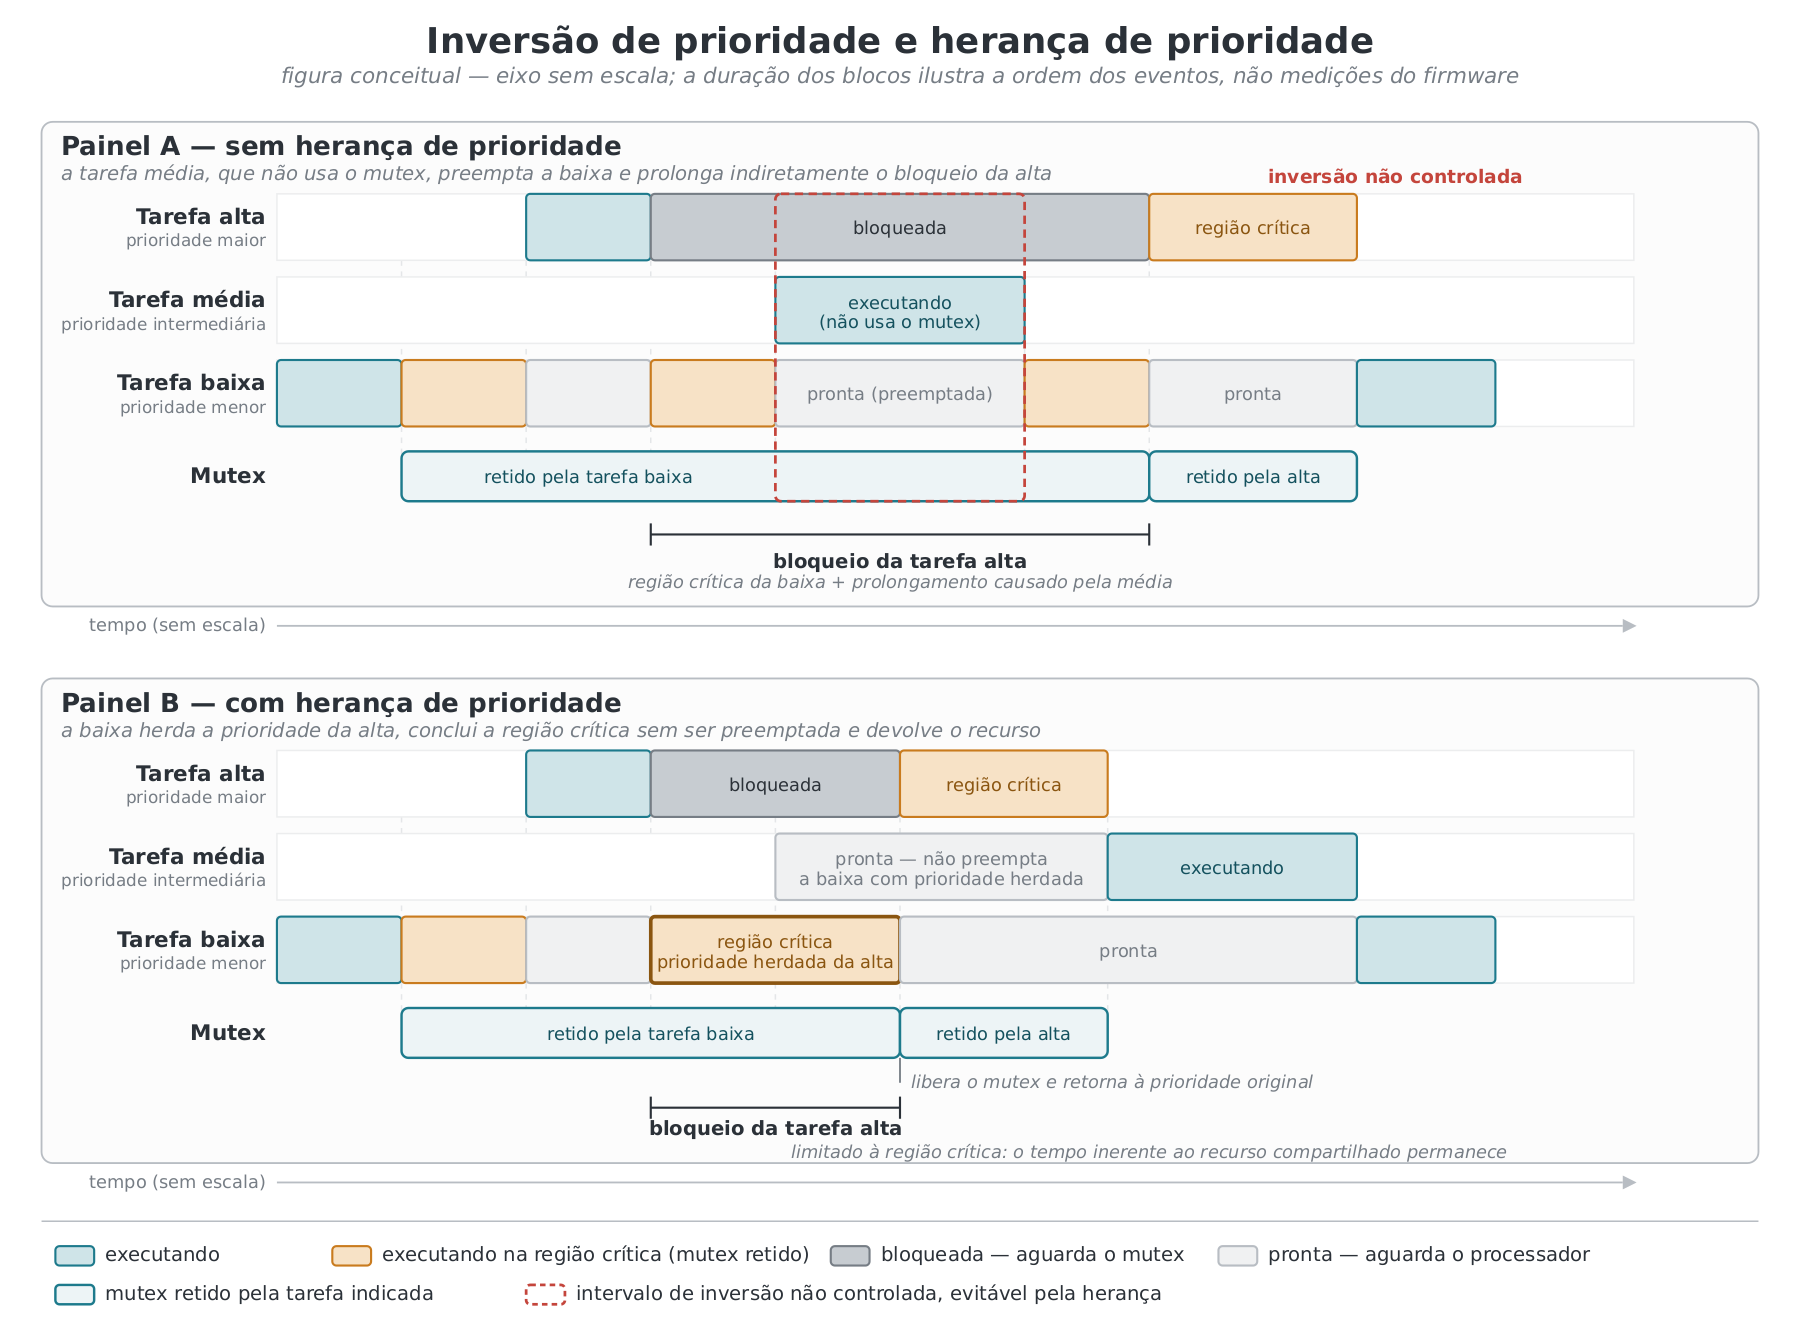
\includegraphics[width=0.94\textwidth]{inversao_prioridade.png}
\fonteelemento{Elaborado pelo autor com base em Sha, Rajkumar e Lehoczky (1990)}
\end{figure}


\subsubsection{Watchdog e carga do processador}


Um temporizador de supervis\~ao, ou \emph{watchdog}, detecta situa\c{c}\~oes em que uma parte do sistema deixa de progredir dentro de um intervalo estabelecido. No ESP-IDF, o watchdog de interrup\c{c}\~oes verifica per\'iodos prolongados em que as interrup\c{c}\~oes e a troca de tarefas n\~ao conseguem ocorrer, enquanto o watchdog de tarefas pode monitorar tarefas inscritas e a execu\c{c}\~ao da tarefa ociosa. A aus\^encia prolongada de execu\c{c}\~ao da tarefa ociosa \'e um ind\'icio de que alguma tarefa n\~ao est\'a cedendo o processador (ESPRESSIF SYSTEMS, 2025d).


O disparo de um watchdog identifica uma viola\c{c}\~ao temporal, mas n\~ao determina sozinho sua causa. Regi\~oes cr\'iticas extensas, interrup\c{c}\~oes desabilitadas, espera ocupada, processamento excessivo e opera\c{c}\~oes longas sobre mem\'oria n\~ao vol\'atil podem produzir sintomas semelhantes. O limite de supervis\~ao deve ser compat\'ivel com o maior intervalo leg\'itimo de execu\c{c}\~ao, sem ser ampliado apenas para ocultar tarefas que deixam de bloquear ou ceder o processador.


A carga da unidade central de processamento (Central Processing Unit --- CPU) pode ser estimada pelo tempo durante o qual as tarefas permanecem em execu\c{c}\~ao. O FreeRTOS pode acumular estat\'isticas de tempo de execu\c{c}\~ao por tarefa e apresent\'a-las como valores absolutos e percentuais, desde que seja configurada uma base de tempo com resolu\c{c}\~ao adequada (FREERTOS, 2026c). Em uma plataforma de n\'ucleo \'unico, o tempo atribu\'ido \`a tarefa ociosa tamb\'em permite estimar a parcela n\~ao utilizada do processador.


Essas m\'etricas dependem da janela de observa\c{c}\~ao e do estado funcional da aplica\c{c}\~ao. Uma medi\c{c}\~ao realizada com telas est\'aticas ou sensores inativos n\~ao representa necessariamente o pior caso. A coleta de estat\'isticas tamb\'em introduz custo de instrumenta\c{c}\~ao, e o percentual de CPU n\~ao substitui a verifica\c{c}\~ao de lat\^encias e prazos das tarefas cr\'iticas.


Uma estimativa baseada na execu\c{c}\~ao da tarefa ociosa pode indicar a folga global do processador em uma janela, desde que exista uma refer\^encia obtida sob condi\c{c}\~oes equivalentes. Ela n\~ao atribui custo a cada tarefa, n\~ao revela diretamente bloqueios em barramentos e pode variar com interrup\c{c}\~oes, modos funcionais e instrumenta\c{c}\~ao. O \emph{idle hook} deve executar rapidamente e n\~ao pode conter espera bloqueante, pois \'e chamado no contexto da tarefa ociosa (FREERTOS, 2026c).


\subsection{Interfaces de comunica\c{c}\~ao}


Interfaces seriais transferem dados por um n\'umero reduzido de condutores, em contraste com interfaces paralelas que transportam v\'arios bits simultaneamente. A quantidade de sinais, o m\'etodo de endere\c{c}amento, a forma de sincroniza\c{c}\~ao e os mecanismos de confirma\c{c}\~ao variam entre os protocolos. Em uma plataforma com sensores e interface gr\'afica, a escolha de cada interface afeta a ocupa\c{c}\~ao de pinos, a taxa de transfer\^encia, a complexidade el\'etrica e a coordena\c{c}\~ao do acesso por software.


\subsubsection{I$^2$C}


O barramento Inter-Integrated Circuit (I$^2$C) utiliza duas linhas: dados seriais (Serial Data --- SDA) e clock serial (Serial Clock --- SCL). As linhas empregam sa\'idas de dreno aberto ou coletor aberto e resistores de \emph{pull-up}. Os dispositivos conectados podem for\c{c}ar uma linha ao n\'ivel baixo, mas o n\'ivel alto resulta da libera\c{c}\~ao coletiva da linha e da a\c{c}\~ao dos resistores. Essa caracter\'istica permite compartilhar os mesmos condutores sem que duas sa\'idas ativas imponham n\'iveis l\'ogicos opostos (NXP SEMICONDUCTORS, 2021).


A comunica\c{c}\~ao \'e organizada em transa\c{c}\~oes iniciadas por uma condi\c{c}\~ao de START e encerradas por uma condi\c{c}\~ao de STOP ou por um START repetido. Ap\'os o endere\c{c}o e a indica\c{c}\~ao de leitura ou escrita, os dados s\~ao transmitidos em grupos de oito bits. Cada byte \'e seguido por um bit de reconhecimento: ACK indica que o receptor reconheceu a transfer\^encia, enquanto NACK pode sinalizar aus\^encia do dispositivo, impossibilidade de receber mais dados ou t\'ermino de uma leitura, conforme a etapa da transa\c{c}\~ao.


V\'arios dispositivos podem compartilhar SDA e SCL, desde que seus endere\c{c}os n\~ao entrem em conflito e que as caracter\'isticas el\'etricas permane\c{c}am dentro dos limites do barramento. O tempo de subida depende da resist\^encia de \emph{pull-up} e da capacit\^ancia total do barramento, formada por dispositivos, trilhas, fios e conectores. O aumento da capacit\^ancia torna as transi\c{c}\~oes para o n\'ivel alto mais lentas e pode limitar a frequ\^encia utiliz\'avel, sendo necess\'ario dimensionar o resistor de \emph{pull-up} de modo a atender simultaneamente ao tempo m\'aximo de subida e \`a corrente que os dispositivos devem drenar quando a linha est\'a em n\'ivel baixo. A Figura~\ref{fig:i2c-open-drain} relaciona o comportamento de dreno aberto \`a subida determinada pela rede resistivo-capacitiva.


\begin{figure}[H]
\centering
\caption{Linha I$^2$C em dreno aberto e subida determinada pela rede de \emph{pull-up} e pela capacit\^ancia equivalente}
\label{fig:i2c-open-drain}
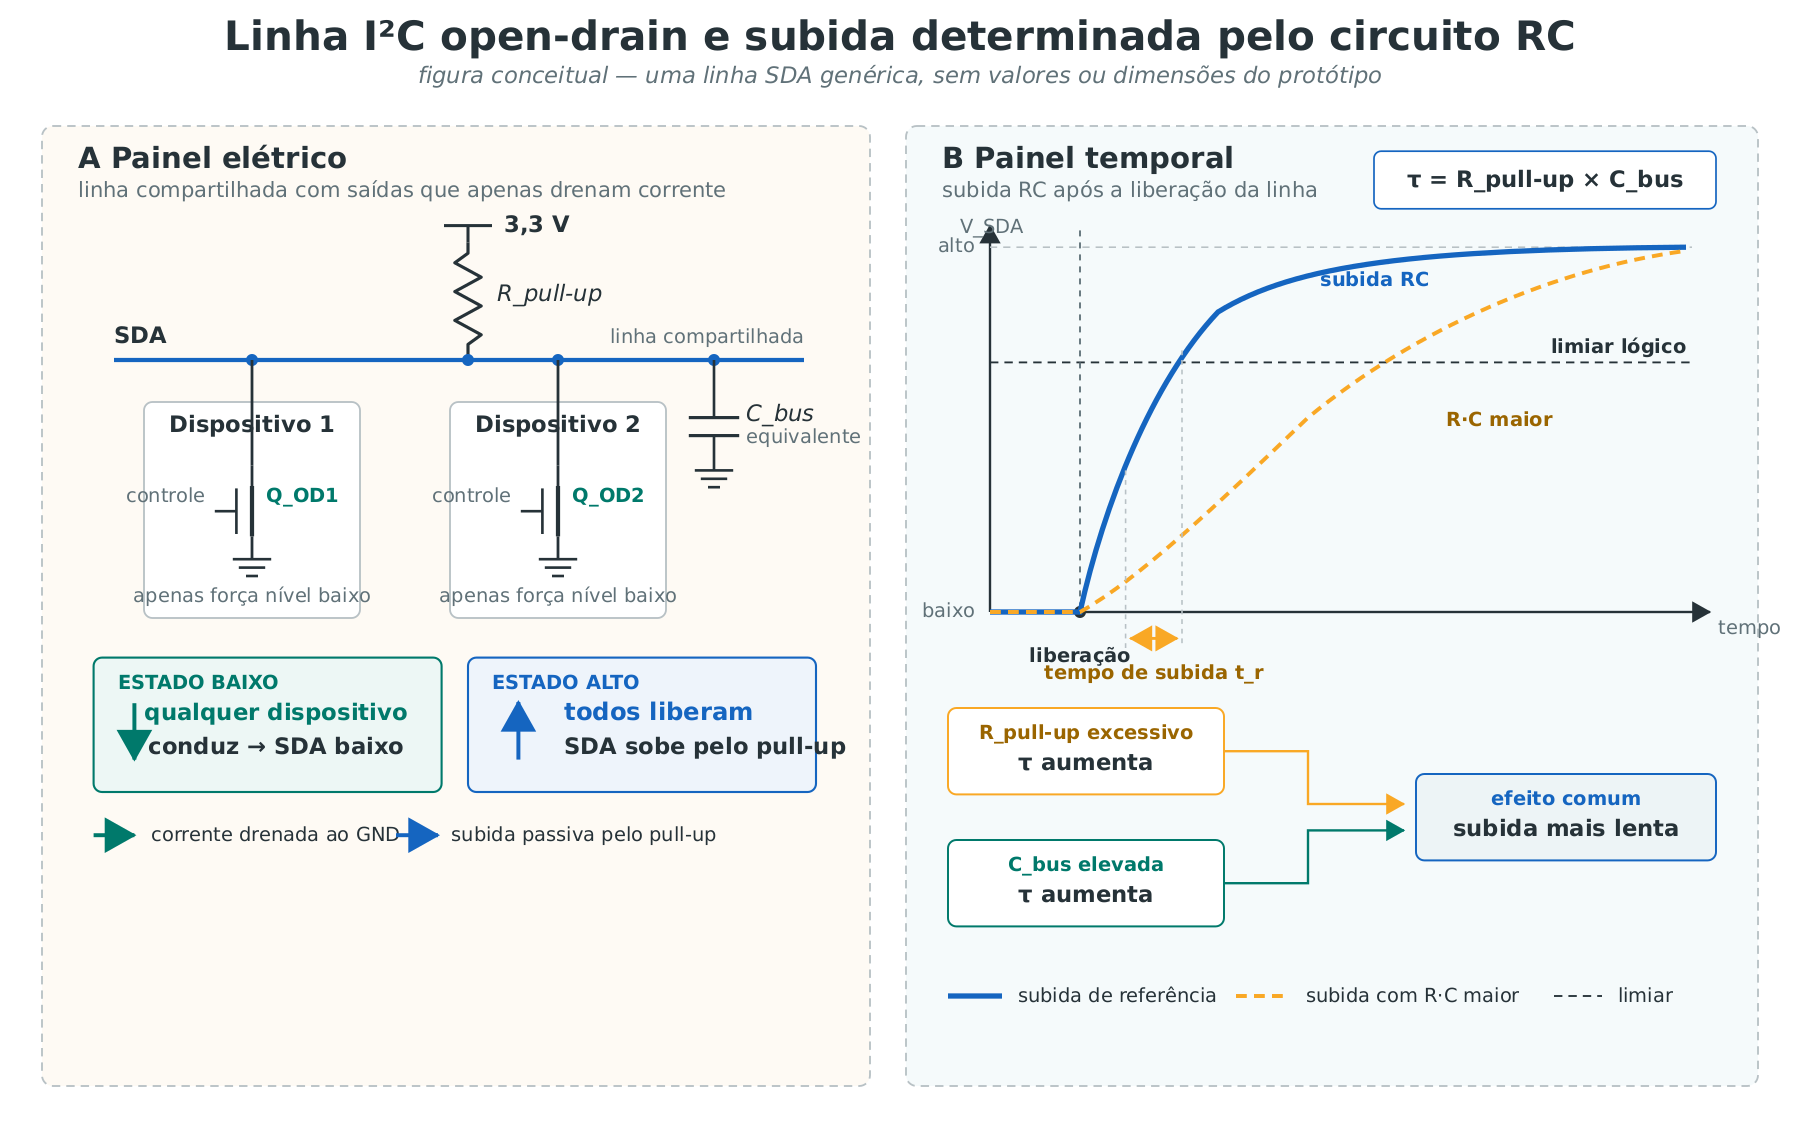
\includegraphics[width=0.94\textwidth]{i2c_open_drain_rc.png}
\fonteelemento{Elaborado pelo autor com base em NXP Semiconductors (2021)}
\end{figure}


O protocolo tamb\'em prev\^e arbitragem para situa\c{c}\~oes em que mais de um controlador pode iniciar transfer\^encias. Alguns dispositivos podem prolongar o n\'ivel baixo de SCL para adiar a continua\c{c}\~ao da transa\c{c}\~ao, recurso denominado \emph{clock stretching}. O suporte efetivo a esses recursos depende dos controladores e dispositivos empregados.


O compartilhamento f\'isico n\~ao fornece exclus\~ao m\'utua entre tarefas de software. Quando diferentes tarefas iniciam transa\c{c}\~oes pelo mesmo controlador, o driver ou a aplica\c{c}\~ao deve preservar a atomicidade de cada opera\c{c}\~ao e impedir que sequ\^encias pertencentes a dispositivos distintos sejam intercaladas. Erros como NACK, limite de espera e barramento ocupado precisam ser tratados de acordo com o estado reportado pelo controlador.


A especifica\c{c}\~ao define, entre outros, o modo padr\~ao de at\'e 100 kbit/s e o modo r\'apido de at\'e 400 kbit/s (NXP SEMICONDUCTORS, 2021). Operar a 100 kbit/s em uma integra\c{c}\~ao e a 400 kbit/s em um teste isolado constitui uma decis\~ao de configura\c{c}\~ao condicionada pelos dispositivos, pela interliga\c{c}\~ao e pelas margens temporais; n\~ao implica que uma das frequ\^encias seja universalmente correta. Ap\'os falhas, a recupera\c{c}\~ao pode exigir encerrar ou reinicializar a transa\c{c}\~ao e o controlador, ou liberar uma linha retida segundo as capacidades do hardware. A estrat\'egia deve evitar que uma tentativa local de recupera\c{c}\~ao interfira em outra transa\c{c}\~ao v\'alida no mesmo barramento.


\subsubsection{SPI}


A Serial Peripheral Interface (SPI) \'e uma interface serial s\'incrona na qual um controlador fornece o sinal de clock e seleciona o dispositivo participante da transa\c{c}\~ao. Na configura\c{c}\~ao convencional, s\~ao utilizados o clock serial (Serial Clock --- SCLK), a linha de dados do controlador para o perif\'erico (Master Out, Slave In --- MOSI), a linha de retorno (Master In, Slave Out --- MISO) e um sinal de sele\c{c}\~ao, usualmente denominado Chip Select (CS), para cada dispositivo.


Como MOSI e MISO s\~ao linhas distintas, a transfer\^encia pode ocorrer simultaneamente nas duas dire\c{c}\~oes. Aplica\c{c}\~oes que necessitam apenas de escrita ou apenas de leitura podem omitir uma das linhas. Diferentemente do I$^2$C, a forma convencional de SPI n\~ao inclui endere\c{c}amento no barramento nem um bit padronizado de reconhecimento a cada byte. O significado dos bits transferidos, a organiza\c{c}\~ao de comandos e a indica\c{c}\~ao de erros s\~ao definidos pelo protocolo do dispositivo.


A rela\c{c}\~ao entre a polaridade do clock e a borda usada para lan\c{c}ar ou amostrar os dados determina o modo SPI. Controlador e perif\'erico precisam utilizar combina\c{c}\~oes compat\'iveis de polaridade e fase; uma configura\c{c}\~ao incorreta pode deslocar a amostragem e corromper os dados. Tamb\'em devem ser respeitados os tempos de ativa\c{c}\~ao do CS, propaga\c{c}\~ao e prepara\c{c}\~ao especificados para o perif\'erico.


Dispositivos podem compartilhar SCLK, MOSI e MISO, permanecendo inativos enquanto seus sinais CS n\~ao estiverem selecionados. Cada dispositivo adicional normalmente exige uma linha CS pr\'opria. O controlador precisa impedir a sobreposi\c{c}\~ao de transa\c{c}\~oes e aplicar a configura\c{c}\~ao de clock e modo correspondente ao dispositivo selecionado. No driver mestre do ESP-IDF, uma transa\c{c}\~ao compreende a sele\c{c}\~ao por CS, a transfer\^encia e a libera\c{c}\~ao do dispositivo; o driver tamb\'em pode utilizar acesso direto \`a mem\'oria para transferir blocos sem movimentar cada byte diretamente pela CPU (ESPRESSIF SYSTEMS, 2025e).


\subsubsection{1-Wire}


O 1-Wire \'e um protocolo serial bidirecional que utiliza uma linha de dados, al\'em da refer\^encia de terra, para comunica\c{c}\~ao entre um controlador e um ou mais dispositivos. A linha \'e compartilhada e mantida em n\'ivel alto por um resistor de \emph{pull-up}; controlador e dispositivos sinalizam ao for\c{c}\'a-la temporariamente ao n\'ivel baixo. Alguns dispositivos podem obter energia da pr\'opria linha quando ela permanece em n\'ivel alto, modalidade denominada alimenta\c{c}\~ao parasita, enquanto outros admitem alimenta\c{c}\~ao externa (ANALOG DEVICES, 2008).


Uma comunica\c{c}\~ao come\c{c}a com um pulso de reinicializa\c{c}\~ao produzido pelo controlador. Os dispositivos presentes respondem com um pulso de presen\c{c}a, ap\'os o qual s\~ao transmitidos comandos de endere\c{c}amento e de fun\c{c}\~ao. Cada dispositivo possui um identificador de 64 bits, que permite selecionar uma unidade espec\'ifica, selecionar todas as unidades ou executar um procedimento de busca no barramento (ANALOG DEVICES, 2019).


Os bits s\~ao representados por intervalos temporais durante os quais o controlador e o dispositivo alteram ou amostram o n\'ivel da linha. H\'a intervalos distintos para escrita de zero, escrita de um e leitura, al\'em de tempos m\'inimos de recupera\c{c}\~ao. Como a interpreta\c{c}\~ao depende da dura\c{c}\~ao dos pulsos e do instante de amostragem, atrasos introduzidos pelo software ou por interrup\c{c}\~oes podem violar os limites do protocolo. No DS18B20, por exemplo, cada intervalo transporta um bit, e o controlador inicia todos os sinais, exceto o pulso de presen\c{c}a (ANALOG DEVICES, 2019).


A redu\c{c}\~ao do n\'umero de condutores ocorre em troca de menor taxa de transfer\^encia e de requisitos temporais estritos. A capacit\^ancia da linha, o valor do resistor de \emph{pull-up}, a topologia da conex\~ao e a quantidade de dispositivos influenciam os tempos de subida e a margem dispon\'ivel para amostragem.


\subsubsection{RMT}


O Remote Control Transceiver (RMT) \'e um perif\'erico para transmiss\~ao e recep\c{c}\~ao de sinais definidos por n\'iveis l\'ogicos e dura\c{c}\~oes. Embora tenha sido concebido para sinais de controle remoto por infravermelho, seu formato permite representar outros protocolos baseados em pulsos. Cada s\'imbolo associa dois n\'iveis a seus respectivos intervalos de dura\c{c}\~ao, e canais independentes podem ser configurados para transmiss\~ao ou recep\c{c}\~ao (ESPRESSIF SYSTEMS, 2025f).


O RMT n\~ao define endere\c{c}os, comandos ou regras de um protocolo de comunica\c{c}\~ao. Ele fornece os recursos temporais usados para produzir ou medir a forma de onda. Um codificador ou driver de n\'ivel superior continua respons\'avel por converter comandos e dados nos s\'imbolos correspondentes e por interpretar os pulsos recebidos.


Ao transferir a gera\c{c}\~ao e a medi\c{c}\~ao dos pulsos para um perif\'erico, reduz-se a depend\^encia de la\c{c}os de software executados com temporiza\c{c}\~ao precisa. Essa separa\c{c}\~ao \'e \'util quando o processador tamb\'em atende tarefas e interrup\c{c}\~oes que poderiam introduzir varia\c{c}\~ao nos instantes de altera\c{c}\~ao ou amostragem de uma entrada ou sa\'ida digital.


\subsection{Interface gr\'afica embarcada}


\subsubsection{TFT e RGB565}


Displays de transistores de filme fino (Thin-Film Transistor --- TFT) empregam uma matriz ativa para controlar os elementos da imagem. Em m\'odulos embarcados, um controlador integrado recebe comandos e dados de pixels, mant\'em a informa\c{c}\~ao na mem\'oria do display e atualiza a matriz. A aplica\c{c}\~ao n\~ao precisa transmitir continuamente o quadro completo para preservar uma imagem est\'atica, mas deve enviar os pixels correspondentes \`as regi\~oes que pretende modificar.


No formato RGB565, cada pixel \'e representado por 16 bits: cinco para vermelho, seis para verde e cinco para azul. Essa codifica\c{c}\~ao oferece \(2^{16}\), ou 65.536, combina\c{c}\~oes poss\'iveis e ocupa dois bytes por pixel. O canal verde recebe um bit adicional porque a sensibilidade visual n\~ao \'e igual para as tr\^es componentes. Em compara\c{c}\~ao com representa\c{c}\~oes de 24 ou 32 bits, o RGB565 reduz a mem\'oria e o volume transferido, com menor resolu\c{c}\~ao de cor (GALAXYCORE, 2022).


O tamanho de um quadro sem compress\~ao \'e dado pelo produto entre largura, altura e quantidade de bytes por pixel. Assim, a mem\'oria exigida cresce linearmente com a \'area da imagem e com a profundidade de cor. Em sistemas nos quais o quadro \'e enviado por uma interface serial, esses mesmos fatores tamb\'em afetam o tempo m\'inimo de transfer\^encia.


\subsubsection{Displays circulares}


Um display circular pode ser controlado por uma matriz de endere\c{c}amento retangular que cont\'em pixels n\~ao vis\'iveis nos cantos. A aplica\c{c}\~ao continua trabalhando com coordenadas cartesianas, mas somente os pontos internos \`a \'area circular aparecem ao usu\'ario. Para um display de raio \(r\) e centro \((x_c,y_c)\), um ponto \((x,y)\) pertence \`a regi\~ao vis\'ivel quando


\[
(x-x_c)^2+(y-y_c)^2 \leq r^2.
\]


Essa geometria reduz a largura dispon\'ivel nas partes superior e inferior da tela. Elementos adequados ao centro podem ser recortados quando deslocados para essas regi\~oes, ainda que suas coordenadas perten\c{c}am ao ret\^angulo l\'ogico. O projeto da interface deve considerar a extens\~ao completa de textos, imagens e \'areas sens\'iveis ao toque, e n\~ao apenas a posi\c{c}\~ao de seus centros.


O recorte circular tamb\'em influencia a organiza\c{c}\~ao visual. Indicadores perif\'ericos podem acompanhar a borda, enquanto informa\c{c}\~oes que exigem maior largura tendem a ocupar a faixa central. A transforma\c{c}\~ao entre coordenadas de toque e objetos gr\'aficos deve manter a mesma orienta\c{c}\~ao, origem e eventual rota\c{c}\~ao adotadas pelo controlador do display. A Figura~\ref{fig:display-circular} explicita a diferen\c{c}a entre a matriz l\'ogica quadrada, a regi\~ao circular vis\'ivel e a zona central conceitualmente mais segura.


\begin{figure}[H]
\centering
\caption{Geometria de uma \'area circular inscrita em uma matriz l\'ogica quadrada}
\label{fig:display-circular}
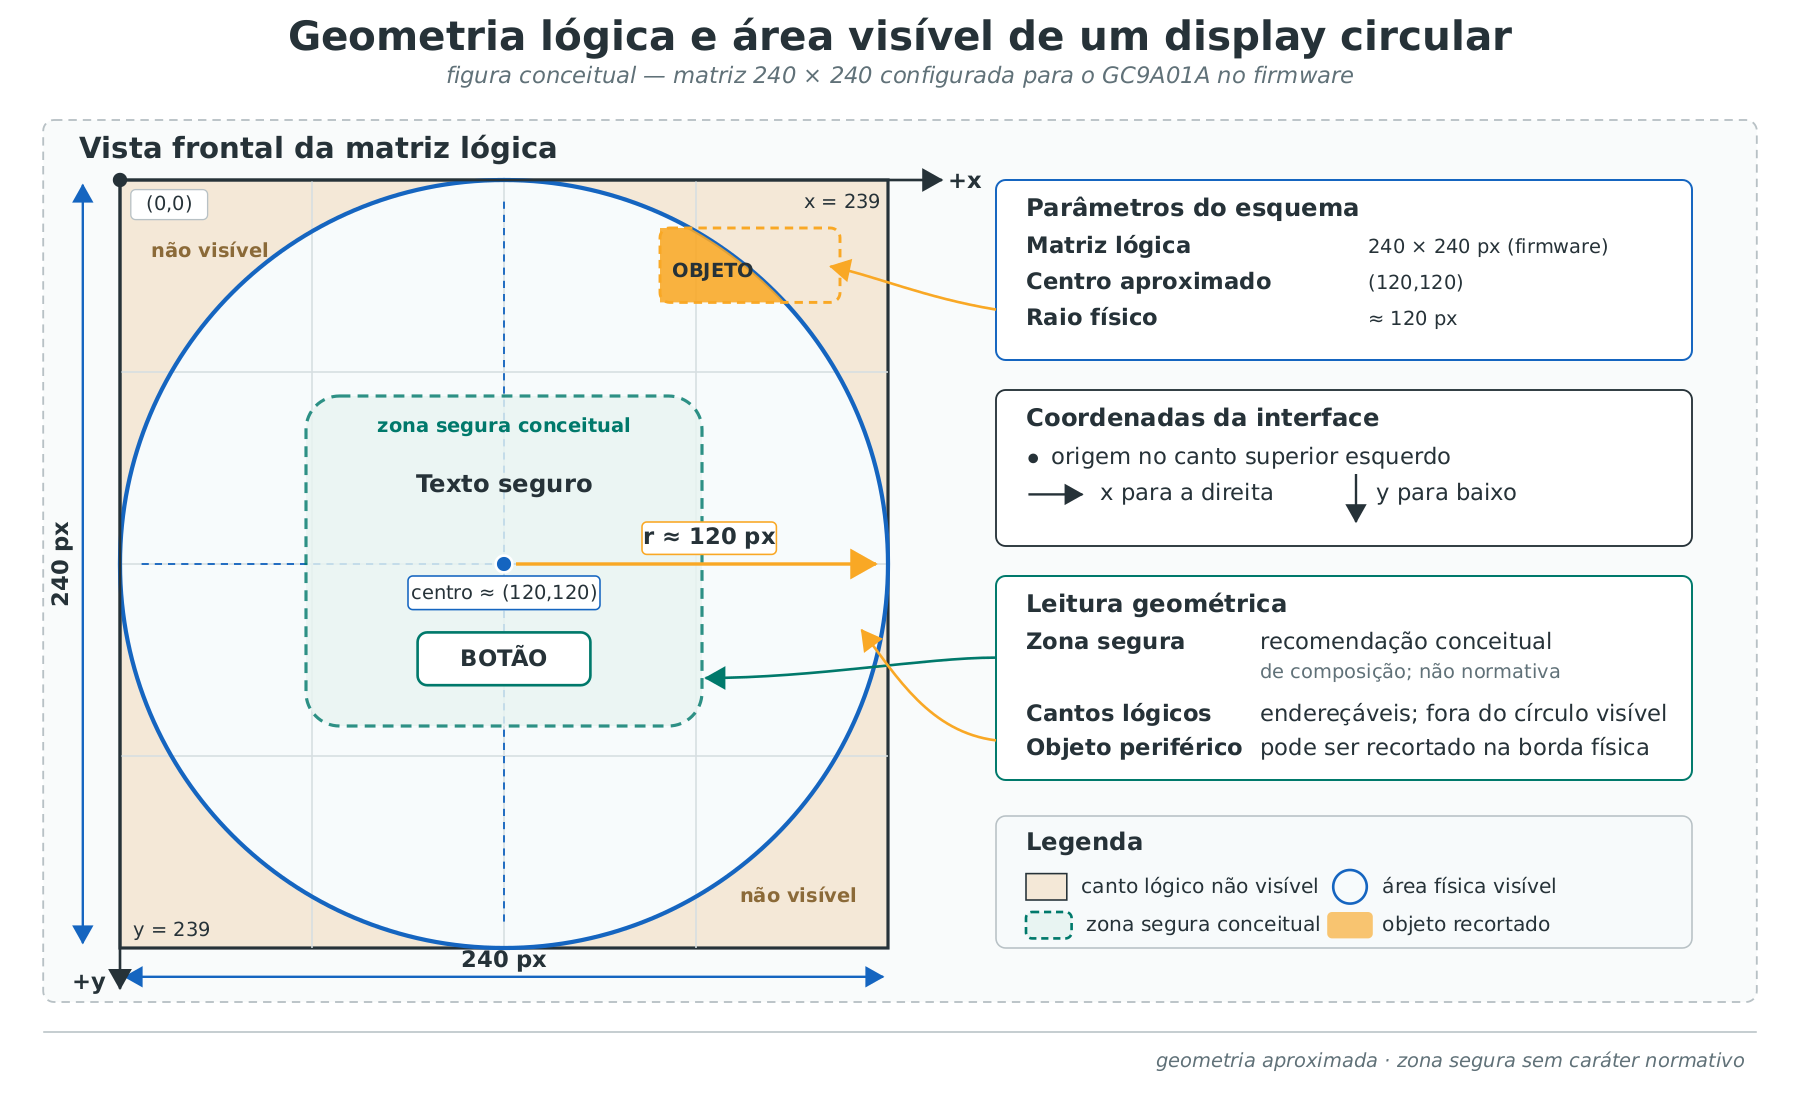
\includegraphics[width=0.90\textwidth]{display_circular_geometria.png}
\fonteelemento{Elaborado pelo autor}
\end{figure}


\subsubsection{LVGL e atualiza\c{c}\~ao parcial}


Bibliotecas gr\'aficas embarcadas, como a Light and Versatile Graphics Library (LVGL), representam a interface por objetos organizados hierarquicamente. Objetos podem conter outros objetos, herdar propriedades e responder a eventos. Essa organiza\c{c}\~ao separa a descri\c{c}\~ao da interface do mecanismo espec\'ifico usado para transferir pixels ao display (LVGL, 2023a).


Quando uma propriedade visual muda, a biblioteca marca como inv\'alidas as regi\~oes afetadas. Durante o ciclo de atualiza\c{c}\~ao, essas regi\~oes s\~ao combinadas quando conveniente, redesenhadas em um buffer e entregues ao driver por uma fun\c{c}\~ao de envio. Dessa forma, uma altera\c{c}\~ao localizada pode ser transmitida sem reconstruir e enviar necessariamente toda a tela (LVGL, 2023b).


O buffer de desenho pode corresponder ao quadro completo ou a uma fra\c{c}\~ao dele. Um buffer parcial reduz a mem\'oria reservada, mas pode exigir v\'arias etapas de desenho e transfer\^encia para concluir uma atualiza\c{c}\~ao. Buffers maiores diminuem a fragmenta\c{c}\~ao da opera\c{c}\~ao, enquanto dois buffers permitem que o processamento de uma regi\~ao se sobreponha \`a transfer\^encia de outra quando o hardware e o driver oferecem esse suporte. A escolha depende da mem\'oria dispon\'ivel, da taxa da interface e da complexidade da cena.


A atualiza\c{c}\~ao parcial reduz trabalho quando poucas regi\~oes mudam, mas seu efeito depende do conte\'udo. Anima\c{c}\~oes extensas, rolagem e objetos transl\'ucidos podem invalidar \'areas maiores e elevar o custo de composi\c{c}\~ao. A taxa de atualiza\c{c}\~ao observada resulta da combina\c{c}\~ao entre desenho, movimenta\c{c}\~ao de mem\'oria, transfer\^encia ao controlador e execu\c{c}\~ao das demais tarefas.


\subsubsection{Mem\'oria de imagens e fontes}


Imagens armazenadas sem compress\~ao consomem mem\'oria proporcionalmente \`as dimens\~oes e \`a profundidade de cor. Uma imagem RGB565 de largura \(L\) e altura \(A\), sem canal adicional, requer \(2LA\) bytes. Metadados, alinhamento e m\'ascaras de transpar\^encia podem acrescentar espa\c{c}o. Formatos comprimidos reduzem o armazenamento, mas exigem decodifica\c{c}\~ao e podem aumentar o tempo de processamento durante a exibi\c{c}\~ao.


Fontes digitais armazenam a representa\c{c}\~ao gr\'afica dos caracteres, denominada glifo, al\'em de m\'etricas de posicionamento. O consumo depende da quantidade de caracteres inclu\'idos, do tamanho, da profundidade de bits e de informa\c{c}\~oes como \emph{kerning}. Incluir todos os caracteres de uma fam\'ilia em v\'arios tamanhos pode ocupar mais mem\'oria do que incluir apenas os conjuntos efetivamente utilizados.


Em microcontroladores, imagens e fontes constantes podem permanecer na mem\'oria de programa, enquanto buffers, estados dos objetos e dados tempor\'arios ocupam mem\'oria de acesso aleat\'orio. Essa distin\c{c}\~ao deve ser observada ao avaliar o custo gr\'afico: reduzir o armazenamento de recursos n\~ao implica necessariamente reduzir o buffer de desenho, e vice-versa.


\subsubsection{Toque capacitivo}


Controladores de toque capacitivo estimam altera\c{c}\~oes de capacit\^ancia associadas \`a aproxima\c{c}\~ao ou ao contato do dedo e entregam eventos ou coordenadas ao processador. O mapeamento para a interface depende da orienta\c{c}\~ao, da rota\c{c}\~ao e da origem adotadas pelo display; por isso, o controlador de toque e a biblioteca gr\'afica precisam compartilhar a mesma transforma\c{c}\~ao geom\'etrica.


No modo de consulta peri\'odica (\emph{polling}), o processador verifica o controlador em intervalos definidos, mesmo quando n\~ao h\'a novo toque. Uma linha de interrup\c{c}\~ao pode sinalizar a disponibilidade de um evento e reduzir consultas desnecess\'arias, mas ainda requer leitura posterior dos dados e tratamento de repiques ou eventos acumulados conforme o controlador. A escolha depende da interface el\'etrica, da lat\^encia desejada, da taxa de consultas e das capacidades do componente; interrup\c{c}\~ao n\~ao elimina a necessidade de coordenar o barramento compartilhado.


\subsubsection{Rel\'ogio de tempo real}


Um rel\'ogio de tempo real (Real-Time Clock --- RTC) mant\'em contagem de segundos e calend\'ario independentemente da atualiza\c{c}\~ao da interface. O PCF8563 utiliza um cristal de 32,768 kHz, comunica-se por I$^2$C e inclui detector de baixa tens\~ao (NXP SEMICONDUCTORS, 2026). Uma fonte de backup pode preservar a oscila\c{c}\~ao e os registradores quando a alimenta\c{c}\~ao principal \'e removida, desde que a placa implemente a comuta\c{c}\~ao adequada.


O erro de frequ\^encia costuma ser expresso em partes por milh\~ao (ppm). Se o erro relativo for aproximadamente constante, um desvio de \(e\) ppm produz, em primeira aproxima\c{c}\~ao, erro temporal de \(e\times10^{-6}\) segundos por segundo. Temperatura, carga capacitiva e envelhecimento do cristal alteram essa taxa; ajustar data e hora na interface n\~ao corrige automaticamente a frequ\^encia do oscilador. O bit de baixa tens\~ao informa que a integridade do calend\'ario pode ter sido comprometida e deve ser verificado antes de tratar a leitura como v\'alida.


\subsection{Bateria, alimenta\c{c}\~ao e convers\~ao anal\'ogico-digital}


\subsubsection{C\'elula recarreg\'avel e estado de carga}


Uma c\'elula de \'ions de l\'itio ou de pol\'imero de l\'itio em configura\c{c}\~ao 1S fornece tens\~ao vari\'avel ao longo da carga e da descarga. A tens\~ao nominal identifica uma regi\~ao de opera\c{c}\~ao da qu\'imica e n\~ao o valor constante nos terminais; os limites de carga, descarga e corrente devem ser obtidos para a c\'elula e o circuito de prote\c{c}\~ao empregados. O carregador controla o processo de carga, enquanto o regulador adapta a tens\~ao da c\'elula aos circuitos do sistema.


Estado de carga (State of Charge --- SoC) \'e a fra\c{c}\~ao da carga remanescente em rela\c{c}\~ao \`a capacidade considerada. A tens\~ao terminal n\~ao determina univocamente o SoC: ela depende tamb\'em da corrente, temperatura, hist\'orico e relaxa\c{c}\~ao da c\'elula. Durante alimenta\c{c}\~ao por USB ou sob carga din\^amica, a interpreta\c{c}\~ao direta da tens\~ao torna-se ainda mais dependente do circuito e do instante da amostra. Um indicador baseado somente em tens\~ao deve, portanto, ser tratado como estimativa aproximada (ANALOG DEVICES, 2006).


Na contagem de coulombs, a corrente que entra e sai da bateria \'e integrada ao longo do tempo. Esse m\'etodo mede fluxo de carga, mas acumula erros de offset e exige uma condi\c{c}\~ao inicial ou corre\c{c}\~oes peri\'odicas. Medidores mais completos combinam tens\~ao, corrente, temperatura e modelos da c\'elula. Estimar autonomia apenas pela divis\~ao entre capacidade nominal e corrente m\'edia pressup\~oe carga constante e capacidade integralmente utiliz\'avel; trata-se de c\'alculo simplificado, n\~ao de uma curva de descarga medida.


\subsubsection{Divisor resistivo e ADC}


Um divisor resistivo permite reduzir a tens\~ao da bateria \`a faixa admiss\'ivel do conversor anal\'ogico-digital (Analog-to-Digital Converter --- ADC). Para resistores \(R_1\) e \(R_2\), com \(R_1\) entre a fonte e o n\'o medido e \(R_2\) entre o n\'o e a refer\^encia,


\[
V_{\mathrm{ADC}}=V_{\mathrm{bat}}\frac{R_2}{R_1+R_2}.
\]


Resist\^encias menores oferecem menor imped\^ancia ao circuito de amostragem, mas drenam corrente continuamente. Resist\^encias maiores reduzem esse consumo e tornam a leitura mais sens\'ivel \`a corrente de entrada, \`a capacit\^ancia de amostragem, a fugas e a interfer\^encias. O compromisso depende do ADC, da taxa de leitura e da possibilidade de comutar o divisor. O dimensionamento e a topologia efetivamente montada pertencem ao cap\'itulo de Desenvolvimento.


O ADC SAR do ESP32-C6 apresenta varia\c{c}\~oes e n\~ao idealidades que impedem converter contagens em tens\~ao por uma rela\c{c}\~ao ideal universal. A atenua\c{c}\~ao define a faixa de entrada e integra a configura\c{c}\~ao da calibra\c{c}\~ao. No ESP-IDF, o ESP32-C6 oferece o esquema de calibra\c{c}\~ao por ajuste de curva (\emph{curve fitting}), que usa par\^ametros do dispositivo para converter a leitura bruta em tens\~ao (ESPRESSIF SYSTEMS, 2025c). A m\'edia de amostras pode reduzir ru\'ido aleat\'orio n\~ao correlacionado, mas n\~ao corrige ganho, offset ou n\~ao linearidade sistem\'aticos.


Backlight, reguladores, carregador, sensores e interface consomem energia em regimes diferentes. A corrente quiescente dos circuitos permanece relevante quando as cargas principais est\~ao reduzidas, e uma fonte de backup do RTC deve ser distinguida da bateria principal. A caracteriza\c{c}\~ao de autonomia exige declarar modo funcional, brilho, atividade dos sensores, comunica\c{c}\~ao e condi\c{c}\~ao de carga.


\subsection{Sensoriamento \'optico biom\'edico}


\subsubsection{Fotopletismografia}


A fotopletismografia (Photoplethysmography --- PPG) \'e uma t\'ecnica \'optica que registra varia\c{c}\~oes associadas ao volume sangu\'ineo no tecido. Uma fonte luminosa ilumina a regi\~ao medida e um fotodetector converte a luz recebida em sinal el\'etrico. As mudan\c{c}as puls\'ateis da perfus\~ao alteram periodicamente a absor\c{c}\~ao e o espalhamento da luz, produzindo uma forma de onda relacionada ao ciclo card\'iaco (ALLEN, 2007).


Na configura\c{c}\~ao transmissiva, fonte e detector ficam em lados opostos do tecido. Na configura\c{c}\~ao reflexiva, ambos ficam no mesmo lado e o detector recebe parte da luz que retorna ap\'os interagir com o tecido. A configura\c{c}\~ao reflexiva \'e compat\'ivel com regi\~oes nas quais n\~ao \'e pr\'atico atravessar completamente o tecido, como o punho, mas sua resposta depende do contato e da geometria \'optica (TAMURA et al., 2014). As duas geometrias s\~ao comparadas na Figura~\ref{fig:ppg-geometrias}.


\begin{figure}[H]
\centering
\caption{Configura\c{c}\~oes transmissiva e reflexiva da fotopletismografia}
\label{fig:ppg-geometrias}
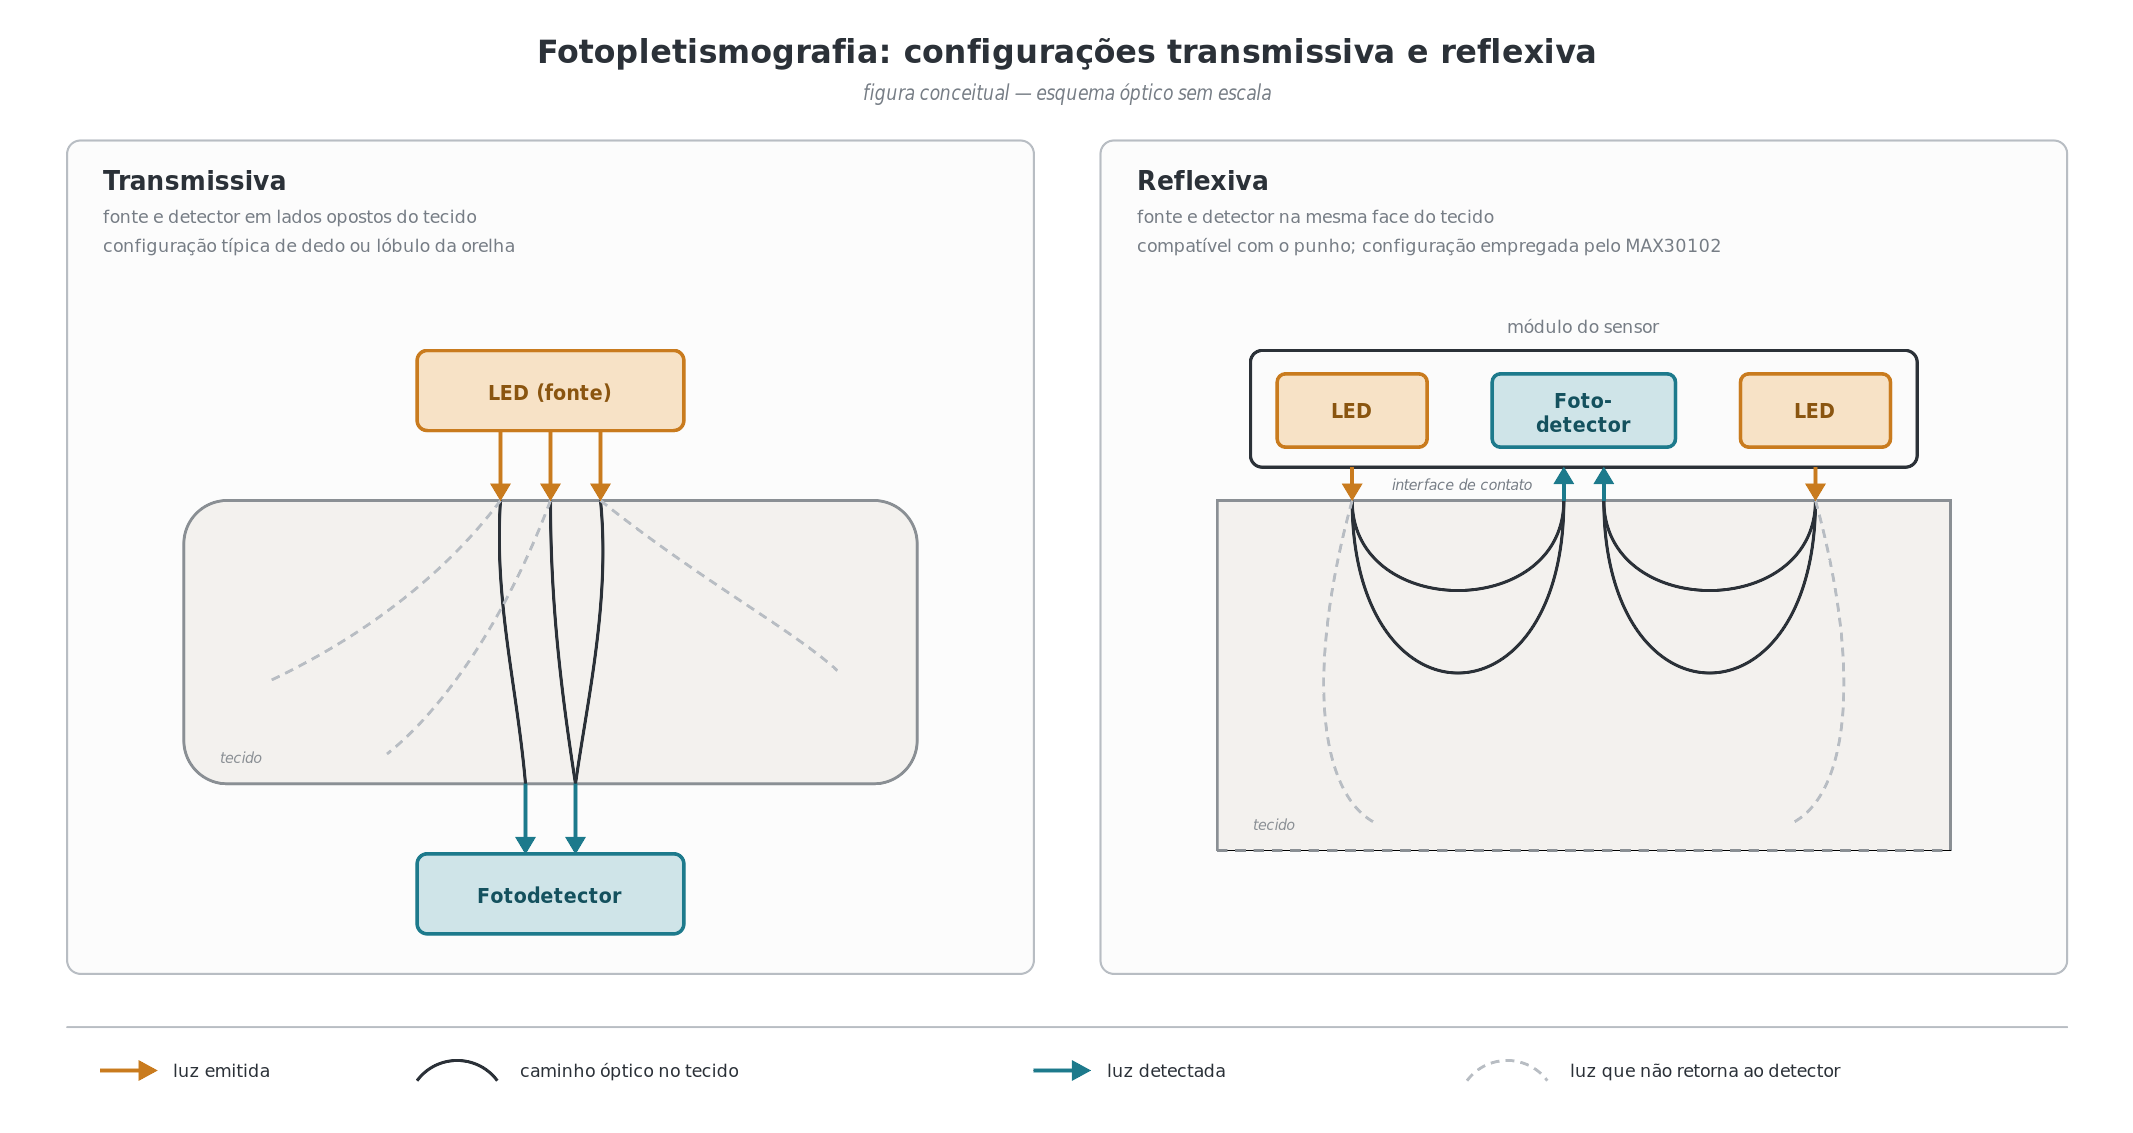
\includegraphics[width=0.94\textwidth]{ppg_transmissiva_reflexiva.png}
\fonteelemento{Elaborado pelo autor com base em Allen (2007), Tamura et al. (2014) e Analog Devices (2018)}
\end{figure}


\subsubsection{Componentes AC e DC}


O sinal PPG pode ser interpretado como a combina\c{c}\~ao de uma componente de varia\c{c}\~ao lenta, usualmente denominada DC, e uma componente puls\'atil, denominada AC. A componente DC re\'une a contribui\c{c}\~ao m\'edia dos tecidos, do sangue n\~ao puls\'atil, da geometria do contato e da intensidade \'optica recebida. A componente AC corresponde \`as varia\c{c}\~oes sincronizadas com a pulsa\c{c}\~ao arterial.


A amplitude AC \'e normalmente muito menor que o n\'ivel DC. O processamento precisa preservar a varia\c{c}\~ao puls\'atil sem saturar a cadeia de aquisi\c{c}\~ao e pode remover tend\^encias lentas para facilitar a detec\c{c}\~ao dos pulsos. Como altera\c{c}\~oes de contato ou movimento tamb\'em modificam o caminho \'optico, a separa\c{c}\~ao espectral n\~ao garante que toda varia\c{c}\~ao na faixa card\'iaca tenha origem fisiol\'ogica. A Figura~\ref{fig:ppg-ac-dc} apresenta essa decomposi\c{c}\~ao em valores normalizados e explicita a diferen\c{c}a de escala da componente puls\'atil.


\begin{figure}[H]
\centering
\caption{Decomposi\c{c}\~ao conceitual do sinal PPG em componentes DC e AC}
\label{fig:ppg-ac-dc}
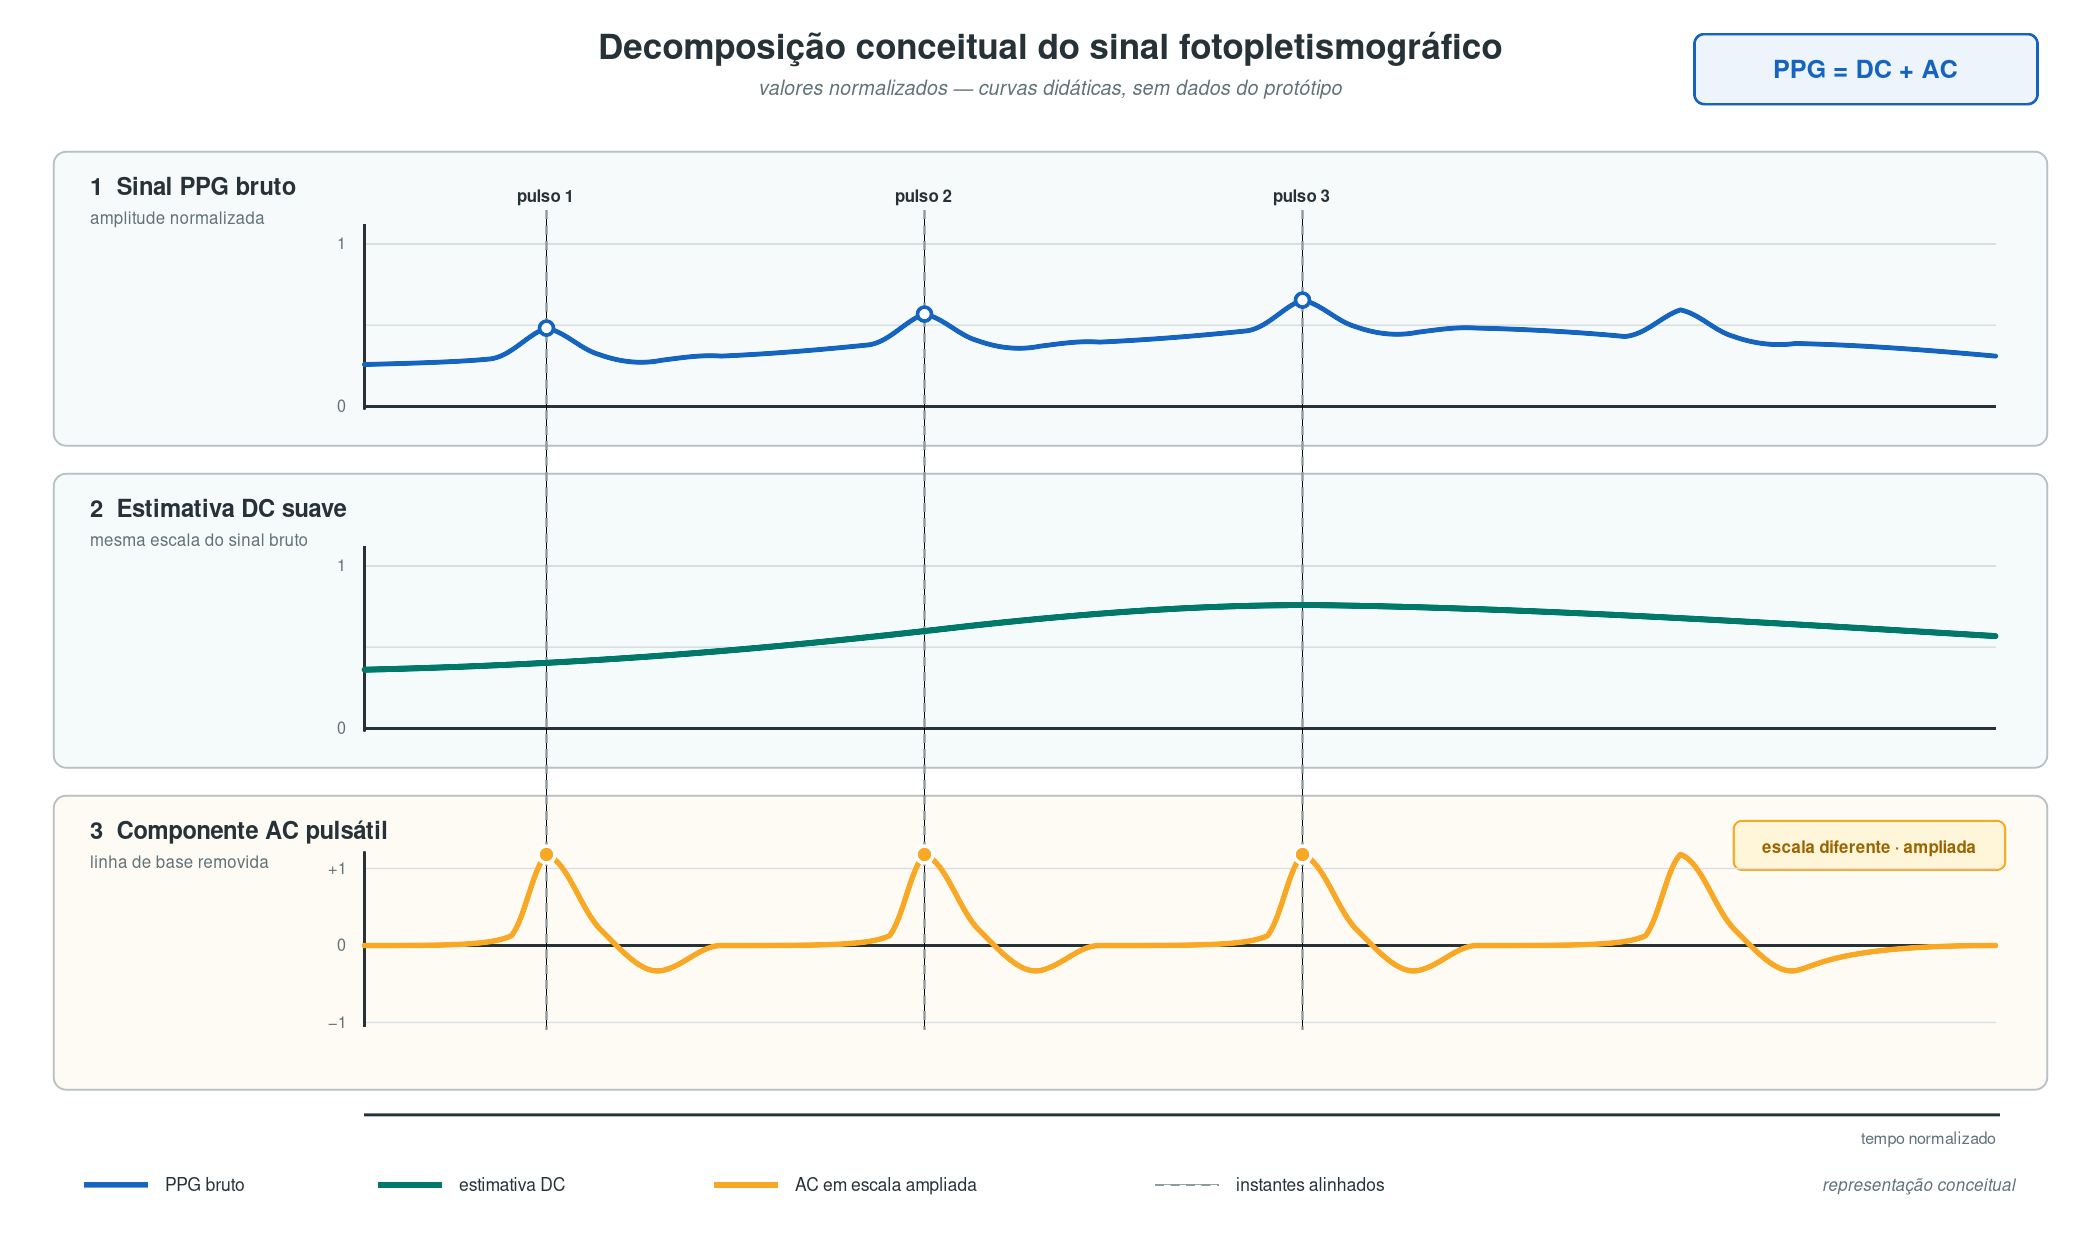
\includegraphics[width=0.94\textwidth]{ppg_componentes_ac_dc.png}
\fonteelemento{Elaborado pelo autor com base em Allen (2007)}
\end{figure}


\subsubsection{Frequ\^encia card\'iaca}


A frequ\^encia card\'iaca pode ser estimada a partir do intervalo entre pulsos consecutivos identificados no sinal PPG. Se \(T\) representa o intervalo m\'edio entre batimentos em segundos, a estimativa em batimentos por minuto \'e


\[
FC=\frac{60}{T}.
\]


O procedimento requer condicionamento do sinal e um crit\'erio para localizar pulsos v\'alidos. Filtragem, limiar, dist\^ancia m\'inima entre picos e rejei\c{c}\~ao de amplitudes incompat\'iveis podem reduzir detec\c{c}\~oes m\'ultiplas e ru\'ido. Esses par\^ametros precisam respeitar a faixa fisiol\'ogica de interesse e a frequ\^encia de amostragem; valores inadequados podem suprimir batimentos reais ou aceitar artefatos como pulsos.


Uma m\'edia calculada sobre v\'arios intervalos reduz a varia\c{c}\~ao da leitura, mas responde mais lentamente a mudan\c{c}as. A frequ\^encia card\'iaca produzida pelo algoritmo \'e uma estimativa dependente da qualidade do sinal e do m\'etodo de detec\c{c}\~ao, e n\~ao uma medi\c{c}\~ao direta da atividade el\'etrica do cora\c{c}\~ao.


\subsubsection{Estimativa de SpO$_2$}


A oximetria de pulso explora a diferen\c{c}a entre os espectros de absor\c{c}\~ao da hemoglobina oxigenada e desoxigenada. A aquisi\c{c}\~ao em dois comprimentos de onda permite comparar a modula\c{c}\~ao puls\'atil observada em cada canal. Uma formula\c{c}\~ao comum utiliza a raz\~ao de raz\~oes


\[
R=\frac{AC_{\mathrm{vermelho}}/DC_{\mathrm{vermelho}}}
        {AC_{\mathrm{infravermelho}}/DC_{\mathrm{infravermelho}}}.
\]


Uma rela\c{c}\~ao emp\'irica converte \(R\) em estimativa da satura\c{c}\~ao perif\'erica de oxig\^enio (SpO$_2$). Embora a lei de Beer--Lambert ajude a descrever a absor\c{c}\~ao em meios homog\^eneos, o tecido biol\'ogico apresenta espalhamento, m\'ultiplos constituintes e caminhos \'opticos vari\'aveis. Por isso, os coeficientes da convers\~ao n\~ao devem ser deduzidos apenas de um modelo ideal; dependem da geometria do sensor, do processamento e de calibra\c{c}\~ao contra valores de refer\^encia (ALLEN, 2007).


A apresenta\c{c}\~ao de uma estimativa de SpO$_2$ n\~ao caracteriza por si s\'o um ox\'imetro validado. O uso cl\'inico exige avalia\c{c}\~ao de exatid\~ao e desempenho segundo procedimentos e faixas apropriados. Sem essa valida\c{c}\~ao, o resultado deve permanecer identificado como estimativa experimental.


\subsubsection{Artefatos e limita\c{c}\~oes}


Movimento relativo entre sensor e pele altera a press\~ao de contato e o caminho percorrido pela luz. O artefato resultante pode ocupar a mesma faixa de frequ\^encias do sinal puls\'atil, o que limita sua remo\c{c}\~ao apenas por filtragem. Luz ambiente que alcan\c{c}a o fotodetector, contato insuficiente, satura\c{c}\~ao, baixa perfus\~ao e varia\c{c}\~oes de pigmenta\c{c}\~ao ou anatomia tamb\'em podem modificar a rela\c{c}\~ao sinal-ru\'ido (TAMURA et al., 2014).


No punho, gestos e marcha produzem componentes peri\'odicas que podem ser confundidas com batimentos. Sensores inerciais podem auxiliar a identificar per\'iodos de movimento, mas n\~ao garantem a reconstru\c{c}\~ao do sinal fisiol\'ogico. A avalia\c{c}\~ao deve incluir o sinal bruto, o sinal processado e condi\c{c}\~oes controladas de repouso e movimento, com registro de perdas de contato ou satura\c{c}\~ao.


As estimativas dependem ainda da taxa de amostragem, da estabilidade temporal, da corrente dos emissores, do ganho do receptor e dos filtros empregados. Compara\c{c}\~oes com um instrumento de refer\^encia precisam utilizar aquisi\c{c}\~ao temporalmente alinhada e popula\c{c}\~ao compat\'ivel com o uso pretendido.


\subsubsection{Aquisi\c{c}\~ao digital e compromissos de configura\c{c}\~ao}


Um sensor integrado como o MAX30102 combina emissores vermelho e infravermelho, fotodetector, eletr\^onica de condicionamento, conversor e fila de primeiro a entrar, primeiro a sair (First In, First Out --- FIFO), comunicando-se por I$^2$C (ANALOG DEVICES, 2018). A FIFO desacopla parcialmente o instante de amostragem do instante em que o processador atende o barramento, mas possui profundidade finita; se n\~ao for drenada a tempo, amostras podem ser sobrescritas ou perdidas conforme a configura\c{c}\~ao.


Taxa de amostragem, largura de pulso, faixa do conversor e corrente dos LEDs formam compromissos de resolu\c{c}\~ao, rela\c{c}\~ao sinal-ru\'ido, consumo e risco de satura\c{c}\~ao. Corrente \'optica maior n\~ao garante sinal utiliz\'avel se o receptor saturar, e faixa maior reduz a chance de satura\c{c}\~ao ao custo da resolu\c{c}\~ao relativa. A ordem dos canais definida pelo componente deve ser confirmada para a placa e o caminho de leitura empregados; uma invers\~ao observada em um m\'odulo espec\'ifico \'e evid\^encia de integra\c{c}\~ao, n\~ao propriedade universal do MAX30102.


\subsection{Sensoriamento de temperatura}


Sensores digitais de temperatura integram o elemento sens\'ivel, a convers\~ao e a interface de comunica\c{c}\~ao, fornecendo a medida em uma representa\c{c}\~ao num\'erica. Essa integra\c{c}\~ao reduz a necessidade de uma cadeia anal\'ogica externa, mas a exatid\~ao permanece condicionada \`as especifica\c{c}\~oes do sensor, \`a faixa de opera\c{c}\~ao, \`a montagem e ao equil\'ibrio t\'ermico com o meio observado.


Resolu\c{c}\~ao e exatid\~ao s\~ao caracter\'isticas distintas. A resolu\c{c}\~ao indica o menor incremento represent\'avel, enquanto a exatid\~ao expressa o limite de erro em rela\c{c}\~ao ao valor verdadeiro nas condi\c{c}\~oes especificadas. Uma leitura com mais casas bin\'arias n\~ao \'e necessariamente mais exata. Em sensores com resolu\c{c}\~ao configur\'avel, maior resolu\c{c}\~ao tamb\'em pode exigir maior tempo de convers\~ao.


Quando a temperatura \'e lida por contato, o encapsulamento, a condu\c{c}\~ao pelas conex\~oes, o fluxo de ar e fontes de calor pr\'oximas influenciam a resposta. Em um dispositivo vest\'ivel, uma medida na regi\~ao do punho n\~ao deve ser tratada automaticamente como temperatura corporal central. C\'odigos de verifica\c{c}\~ao, como a verifica\c{c}\~ao c\'iclica de redund\^ancia (Cyclic Redundancy Check --- CRC), detectam determinadas corrup\c{c}\~oes na comunica\c{c}\~ao, mas n\~ao corrigem erros t\'ermicos ou de posicionamento (ANALOG DEVICES, 2019).


O DS18B20 realiza convers\~ao digital configur\'avel de 9 a 12 bits e armazena o resultado em um \emph{scratchpad} protegido por CRC. O tempo m\'aximo de convers\~ao cresce com a resolu\c{c}\~ao selecionada, de modo que o controlador deve aguardar a conclus\~ao ou consult\'a-la antes de interpretar o resultado. Ap\'os energiza\c{c}\~ao, o registrador de temperatura apresenta 85~$^\circ$C at\'e que uma convers\~ao seja executada; esse valor deve ser interpretado com o estado da opera\c{c}\~ao, e n\~ao aceito isoladamente como temperatura do meio (ANALOG DEVICES, 2019).


O tempo necess\'ario para o encapsulamento aproximar-se da temperatura do objeto constitui resposta t\'ermica e \'e diferente do tempo de convers\~ao digital. Contato mec\^anico, massa t\'ermica, condu\c{c}\~ao pelos fios e convec\c{c}\~ao determinam uma constante de tempo efetiva da montagem. Filtrar ou aumentar a resolu\c{c}\~ao n\~ao acelera esse equil\'ibrio.


\subsection{Sensoriamento \'optico ambiental}


\subsubsection{Ilumin\^ancia}


Ilumin\^ancia \'e a grandeza fotom\'etrica que representa o fluxo luminoso incidente por unidade de \'area, ponderado pela sensibilidade espectral do sistema visual humano. Sua unidade no Sistema Internacional \'e o lux, equivalente a l\'umen por metro quadrado. Por utilizar pondera\c{c}\~ao fot\'opica, a ilumin\^ancia n\~ao corresponde simplesmente \`a pot\^encia \'optica total recebida pelo sensor.


Sensores de luz ambiente aproximam essa resposta por meio de sua sensibilidade espectral e de uma convers\~ao entre contagens digitais e lux. Ganho, tempo de integra\c{c}\~ao e faixa de medida afetam resolu\c{c}\~ao e satura\c{c}\~ao. A rela\c{c}\~ao de convers\~ao fornecida pelo fabricante pressup\~oe condi\c{c}\~oes definidas e pode ser alterada pela janela \'optica, pelo \^angulo de incid\^encia e pelo espectro da fonte (LITE-ON TECHNOLOGY, 2024).


\subsubsection{Radia\c{c}\~ao ultravioleta e UVI}


A radia\c{c}\~ao ultravioleta compreende comprimentos de onda menores que os da luz vis\'ivel. Para comunica\c{c}\~ao do risco da exposi\c{c}\~ao solar, o \'Indice Ultravioleta (Ultraviolet Index --- UVI) representa a irradi\^ancia ultravioleta ponderada pela a\c{c}\~ao eritematosa sobre a pele e escalonada por uma constante. Trata-se de uma grandeza adimensional, n\~ao de uma leitura direta em lux (WORLD HEALTH ORGANIZATION et al., 2002).


Um sensor com canal ultravioleta produz contagens relacionadas \`a radia\c{c}\~ao que alcan\c{c}a sua \'area sens\'ivel. A convers\~ao dessas contagens em UVI depende da resposta espectral, do ganho, do tempo de integra\c{c}\~ao, da calibra\c{c}\~ao e das condi\c{c}\~oes \'opticas de montagem. Barreiras transparentes no vis\'ivel podem atenuar significativamente o ultravioleta (LITE-ON TECHNOLOGY, 2024).


Uma estimativa local produzida por um sensor de baixo custo n\~ao \'e automaticamente equivalente ao UVI meteorol\'ogico. Instrumentos de refer\^encia aplicam resposta espectral e calibra\c{c}\~ao adequadas, enquanto o valor divulgado para uma regi\~ao tamb\'em pode envolver modelos e condi\c{c}\~oes atmosf\'ericas. A interpreta\c{c}\~ao deve conservar essa distin\c{c}\~ao.


\subsubsection{Modos, integra\c{c}\~ao e satura\c{c}\~ao}


O LTR390 compartilha a mesma cadeia de convers\~ao entre um modo de luz ambiente (Ambient Light Sensing --- ALS) e um modo de ultravioleta (Ultraviolet Sensing --- UVS); os dois canais n\~ao s\~ao adquiridos simultaneamente. A altern\^ancia requer configurar o modo e aguardar uma amostra correspondente \`a nova condi\c{c}\~ao. Uma leitura obtida durante a estabiliza\c{c}\~ao n\~ao deve ser misturada ao estado filtrado do outro canal (LITE-ON TECHNOLOGY, 2024).


O ganho multiplica a resposta antes da convers\~ao e favorece sinais pequenos, mas reduz a margem at\'e satura\c{c}\~ao. Maior tempo de integra\c{c}\~ao e resolu\c{c}\~ao podem melhorar a discrimina\c{c}\~ao de contagens, ao custo de menor taxa de atualiza\c{c}\~ao e maior probabilidade de saturar em incid\^encia intensa. Como ALS e UVS representam grandezas e respostas espectrais distintas, cada canal deve manter seus pr\'oprios par\^ametros de convers\~ao e estado de filtragem quando as leituras s\~ao alternadas.


\subsection{Sensoriamento inercial e magn\'etico}


\subsubsection{Aceler\^ometros MEMS}


Um aceler\^ometro baseado em sistemas microeletromec\^anicos (Microelectromechanical Systems --- MEMS) mede acelera\c{c}\~ao espec\'ifica ao longo de um ou mais eixos. Em repouso sobre uma superf\'icie, sua sa\'ida inclui a rea\c{c}\~ao associada ao campo gravitacional; em movimento, combina essa componente com acelera\c{c}\~oes produzidas pela din\^amica do dispositivo. Sensores triaxiais fornecem as componentes \(a_x\), \(a_y\) e \(a_z\) em um sistema de coordenadas fixado ao encapsulamento.


A magnitude


\[
\lVert\mathbf{a}\rVert=\sqrt{a_x^2+a_y^2+a_z^2}
\]


reduz a depend\^encia da orienta\c{c}\~ao dos eixos para detectar varia\c{c}\~oes de intensidade. Ela n\~ao elimina efeitos da posi\c{c}\~ao no corpo, rota\c{c}\~ao do dispositivo, impacto ou movimento do bra\c{c}o. Faixa de medi\c{c}\~ao, resolu\c{c}\~ao, frequ\^encia de amostragem e filtragem tamb\'em condicionam os eventos que podem ser distinguidos.


Desvios constantes, diferen\c{c}as de escala entre eixos, ru\'ido e desalinhamento introduzem erros. A calibra\c{c}\~ao pode estimar parte desses termos a partir de orienta\c{c}\~oes ou refer\^encias conhecidas, mas sua necessidade e seu procedimento dependem da aplica\c{c}\~ao.


Faixa de medi\c{c}\~ao e resolu\c{c}\~ao efetiva formam um compromisso: ampliar a faixa evita satura\c{c}\~ao em impactos, enquanto uma faixa menor atribui mais contagens por unidade de acelera\c{c}\~ao. A taxa de dados de sa\'ida (Output Data Rate --- ODR) limita as varia\c{c}\~oes temporais observ\'aveis e deve ser compat\'ivel com a filtragem aplicada. Filtragem insuficiente pode preservar ru\'ido e aliasing; filtragem excessiva pode atenuar eventos de passo.


O ADXL345 e o aceler\^ometro integrado ao MPU-9250 ilustram componentes capazes de fornecer acelera\c{c}\~ao triaxial, mas n\~ao s\~ao intercambi\'aveis sem considerar faixa, resolu\c{c}\~ao, ODR e interface. Um componente avaliado em prototipagem n\~ao deve ser apresentado como parte da plataforma final se foi substitu\'ido. No MPU-9250, um mesmo encapsulamento re\'une o girosc\'opio e o aceler\^ometro do n\'ucleo MPU-6500 com o magnet\^ometro AK8963 em outro \emph{die} (TDK INVENSENSE, 2016).


\subsubsection{Magnet\^ometros triaxiais}


Um magnet\^ometro triaxial mede as componentes do vetor densidade de fluxo magn\'etico segundo tr\^es eixos ortogonais. Em condi\c{c}\~oes ideais, a orienta\c{c}\~ao do sensor em rela\c{c}\~ao ao campo terrestre altera essas componentes sem alterar a magnitude do vetor. Na pr\'atica, a leitura inclui o campo de interesse, campos produzidos pelo pr\'oprio dispositivo, materiais pr\'oximos e erros do sensor.


O uso do magnet\^ometro como b\'ussola requer conhecer a correspond\^encia entre os eixos f\'isicos e o sistema de coordenadas adotado pelo software. Trocas de eixo e invers\~oes de sinal alteram o sentido angular calculado. A montagem e a orienta\c{c}\~ao gr\'afica precisam, portanto, empregar uma conven\c{c}\~ao comum.


No MPU-9250, o AK8963 pode ser acessado pelo controlador auxiliar interno ou exposto ao barramento principal por um modo de \emph{bypass}. Antes da medi\c{c}\~ao, coeficientes de ajuste de sensibilidade gravados em mem\'oria de fus\'iveis devem ser lidos segundo a sequ\^encia definida pelo fabricante e aplicados por eixo. Esse ajuste de f\'abrica converte a sensibilidade do componente, mas n\~ao substitui a calibra\c{c}\~ao das perturba\c{c}\~oes magn\'eticas introduzidas pela montagem e pelo ambiente (TDK INVENSENSE, 2016; AKM, 2013).


\subsubsection{Campo magn\'etico terrestre}


O campo magn\'etico terrestre pode ser representado por uma componente horizontal e uma componente vertical no local da medi\c{c}\~ao. A dire\c{c}\~ao da componente horizontal define o norte magn\'etico. Ela n\~ao coincide necessariamente com o norte geogr\'afico; o \^angulo entre ambos \'e denominado declina\c{c}\~ao magn\'etica e varia com posi\c{c}\~ao e tempo.


O campo medido no interior de um equipamento pode diferir do campo ambiente. Correntes el\'etricas, \'im\~as, alto-falantes, motores, parafusos e estruturas ferromagn\'eticas produzem perturba\c{c}\~oes. A proximidade de objetos externos tamb\'em pode tornar uma calibra\c{c}\~ao previamente obtida inadequada para aquele ambiente.


\subsubsection{Heading e calibra\c{c}\~ao}


O \emph{heading} \'e o \^angulo de orienta\c{c}\~ao no plano horizontal em rela\c{c}\~ao a uma dire\c{c}\~ao de refer\^encia. Quando o sensor permanece nivelado e os eixos \(x\) e \(y\) correspondem ao plano horizontal, ele pode ser calculado por uma fun\c{c}\~ao de arco tangente com dois argumentos, por exemplo


\[
\psi=\operatorname{atan2}(m_y,m_x).
\]


A ordem dos argumentos, os sinais e o deslocamento angular dependem da conven\c{c}\~ao dos eixos e do sentido positivo adotado. O resultado obtido do campo \'e referido ao norte magn\'etico; a convers\~ao para norte geogr\'afico exige aplicar a declina\c{c}\~ao local.


Perturba\c{c}\~oes aproximadamente constantes no sistema de coordenadas do sensor deslocam o centro da nuvem de medidas e s\~ao associadas ao efeito \emph{hard iron}. Materiais que deformam o campo podem alterar escalas e ortogonalidade, produzindo efeito \emph{soft iron}. Em tr\^es dimens\~oes, uma calibra\c{c}\~ao geral estima um vetor de deslocamento e uma transforma\c{c}\~ao matricial para aproximar a nuvem medida de uma esfera centrada na origem (RENAUDIN; AFZAL; LACHAPELLE, 2010).


Uma calibra\c{c}\~ao baseada somente nos extremos de cada eixo corrige deslocamentos e escalas diagonais, mas n\~ao representa acoplamentos entre eixos. Al\'em disso, o c\'alculo bidimensional sem compensa\c{c}\~ao de inclina\c{c}\~ao pressup\~oe que o sensor permane\c{c}a aproximadamente nivelado. Quando essa condi\c{c}\~ao n\~ao \'e satisfeita, a componente vertical do campo \'e projetada nos eixos usados no c\'alculo e introduz erro angular. A Figura~\ref{fig:calibracao-magnetica} compara as nuvens ideal, deslocada, deformada e corrigida, destacando o alcance limitado da corre\c{c}\~ao diagonal.


\begin{figure}[H]
\centering
\caption{Efeitos de \emph{hard iron} e \emph{soft iron} e alcance da corre\c{c}\~ao diagonal}
\label{fig:calibracao-magnetica}
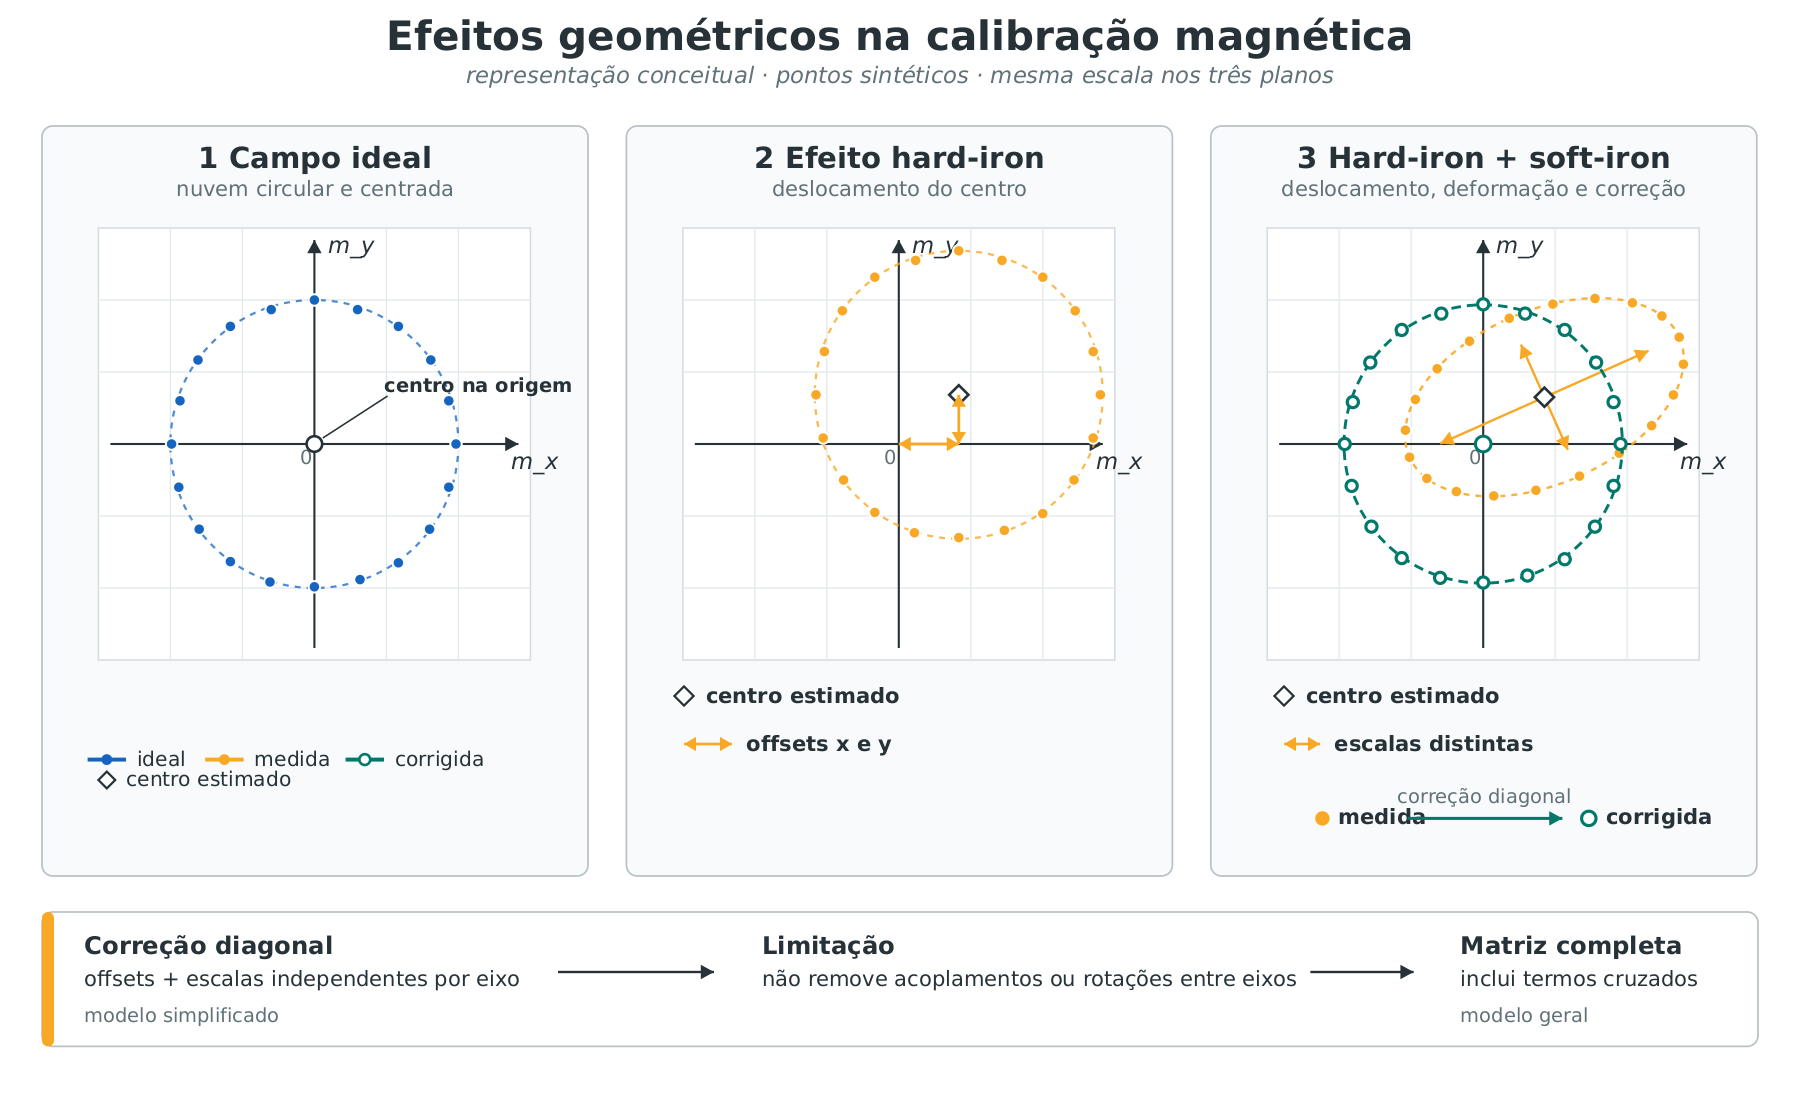
\includegraphics[width=0.94\textwidth]{calibracao_magnetica.png}
\fonteelemento{Elaborado pelo autor com base em Renaudin, Afzal e Lachapelle (2010)}
\end{figure}


A compensa\c{c}\~ao de inclina\c{c}\~ao usa uma estimativa de atitude, normalmente obtida do aceler\^ometro e eventualmente do girosc\'opio, para projetar o vetor magn\'etico no plano horizontal antes do c\'alculo angular. Ela reduz o erro geom\'etrico associado \`a inclina\c{c}\~ao, mas introduz depend\^encia da calibra\c{c}\~ao e da din\^amica dos sensores inerciais. No escopo deste trabalho, esse recurso \'e fundamento para uma extens\~ao futura: o algoritmo final avaliado calcula \emph{heading} bidimensional e pressup\~oe o dispositivo aproximadamente nivelado.


\subsubsection{Marcha e pedometria}


A marcha produz padr\~oes recorrentes de acelera\c{c}\~ao associados \`as fases do passo. Um ped\^ometro procura identificar esses eventos em meio a movimentos que n\~ao correspondem \`a caminhada. M\'etodos simples aplicam filtragem, limiares e busca de picos \`a magnitude da acelera\c{c}\~ao ou a um eixo selecionado.


Um limiar de amplitude rejeita varia\c{c}\~oes pequenas, enquanto um intervalo m\'inimo entre detec\c{c}\~oes evita contar v\'arias oscila\c{c}\~oes do mesmo passo. Limiares fixos podem falhar quando a intensidade da marcha, o usu\'ario ou a posi\c{c}\~ao do dispositivo mudam. Estrat\'egias adaptativas e o uso de caracter\'isticas temporais podem ampliar a faixa de funcionamento, com maior custo e necessidade de parametriza\c{c}\~ao (BRAJDIC; HARLE, 2013).


Uma m\'edia m\'ovel exponencial (Exponential Moving Average --- EMA) de primeira ordem atualiza o estado filtrado por


\[
y_k=\alpha x_k+(1-\alpha)y_{k-1}, \qquad 0<\alpha\leq 1,
\]


em que \(x_k\) \'e a amostra corrente. Valores menores de \(\alpha\) suavizam mais o sinal e aumentam o atraso. Em uma detec\c{c}\~ao por limiar, a histerese usa limites diferentes para armar e confirmar o evento, reduzindo comuta\c{c}\~oes repetidas pr\'oximas ao limiar. Um per\'iodo refrat\'ario rejeita novos eventos por um intervalo ap\'os um passo aceito; ele reduz contagens m\'ultiplas, mas pode suprimir passos reais se for incompat\'ivel com a cad\^encia. A Figura~\ref{fig:pedometro-limiar} relaciona o sinal filtrado, o limiar e o intervalo refrat\'ario na aceita\c{c}\~ao ou rejei\c{c}\~ao de picos.


Movimentos r\'itmicos do bra\c{c}o, transporte do dispositivo fora do punho e vibra\c{c}\~oes podem gerar falsos positivos; passos suaves podem resultar em falsos negativos. A valida\c{c}\~ao exige trajetos ou sequ\^encias controladas, contagem de refer\^encia e condi\c{c}\~oes declaradas de uso. A compara\c{c}\~ao entre passos detectados e passos reais pode ser expressa por erro absoluto, erro relativo e distribui\c{c}\~ao dos erros entre repeti\c{c}\~oes.


\begin{figure}[H]
\centering
\caption{Detec\c{c}\~ao conceitual de passos por limiar e intervalo refrat\'ario}
\label{fig:pedometro-limiar}
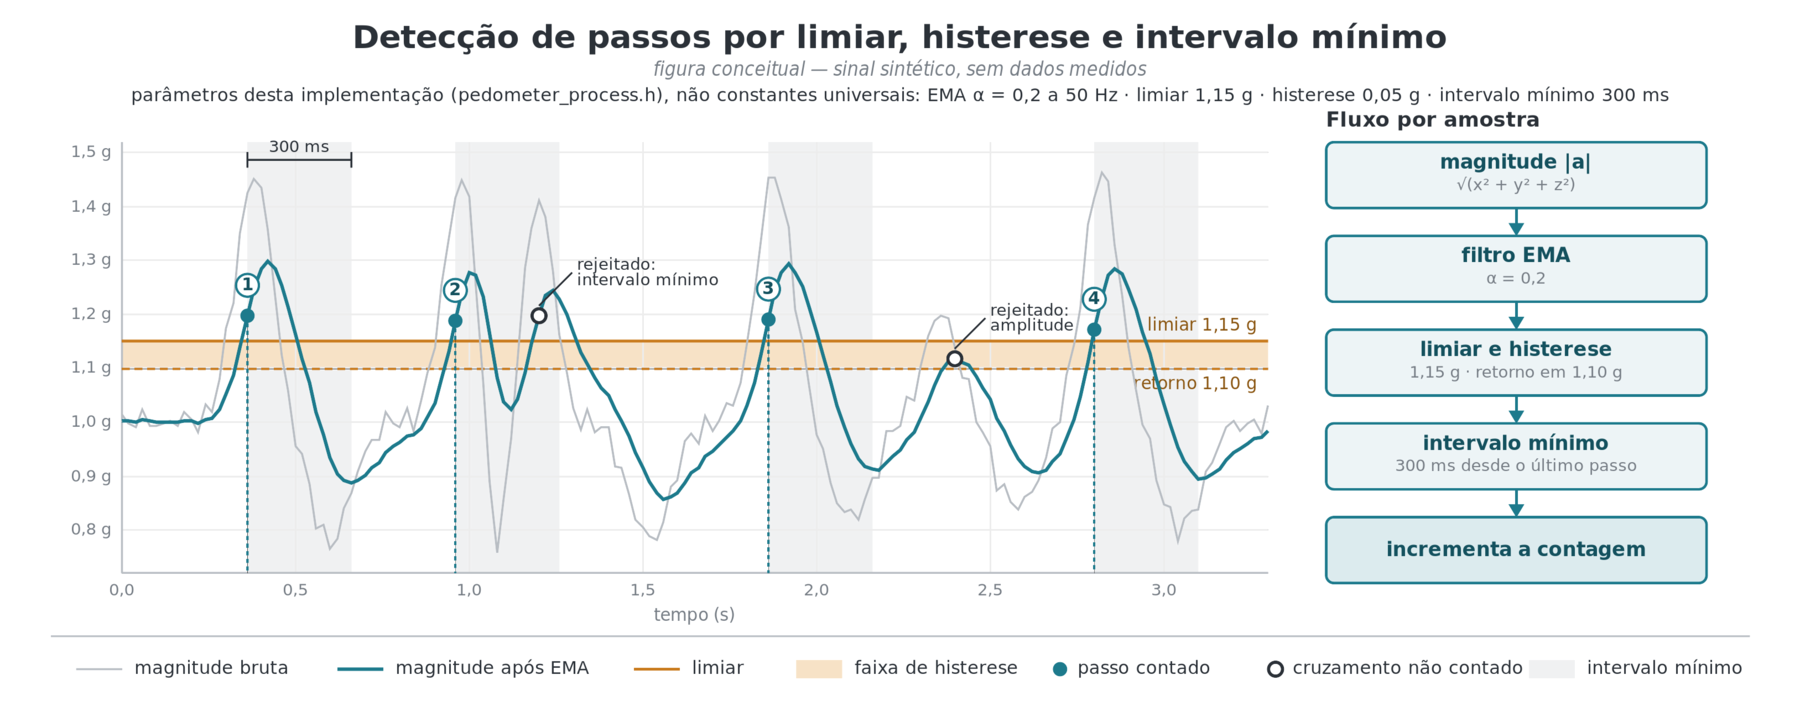
\includegraphics[width=0.94\textwidth]{pedometro_limiar.png}
\fonteelemento{Elaborado pelo autor com base em Brajdic e Harle (2013)}
\end{figure}


\subsection{Trabalhos relacionados}


\subsubsection{Crit\'erios de compara\c{c}\~ao}


Os trabalhos relacionados foram selecionados por apresentarem plataformas vest\'iveis program\'aveis, aquisi\c{c}\~ao multissensor ou organiza\c{c}\~ao destinada a m\'ultiplas aplica\c{c}\~oes. A compara\c{c}\~ao considera plataforma, sistema operacional, sensores, modularidade, extensibilidade, toler\^ancia a falhas, forma de avalia\c{c}\~ao e disponibilidade de c\'odigo. Os termos n\~ao s\~ao tratados como equivalentes quando descrevem n\'iveis distintos: modularidade f\'isica de sensores, modularidade de software e suporte a m\'ultiplas aplica\c{c}\~oes s\~ao registrados separadamente.


\subsubsection{Plataformas vest\'iveis abertas e multissensores}


Hester et al. (2016) apresentam o Amulet, uma plataforma vest\'ivel de baixo consumo destinada \`a execu\c{c}\~ao simult\^anea de aplica\c{c}\~oes. O sistema combina hardware pr\'oprio, sistema operacional e cadeia de ferramentas, com isolamento de mem\'oria e controle de acesso a recursos. A avalia\c{c}\~ao enfatiza consumo de energia e execu\c{c}\~ao de m\'ultiplas aplica\c{c}\~oes. Inclus\~ao de sensores por um contrato uniforme de m\'odulos e continuidade diante da aus\^encia de perif\'ericos n\~ao s\~ao as unidades de an\'alise adotadas nesse estudo.


Baldini et al. (2023) prop\~oem uma plataforma vest\'ivel aberta para aquisi\c{c}\~ao e processamento em tempo real de sinais fisiol\'ogicos. A organiza\c{c}\~ao distribui aquisi\c{c}\~ao, fus\~ao e armazenamento remoto entre blocos conectados e permite integrar diferentes dispositivos de medi\c{c}\~ao. O foco da avalia\c{c}\~ao est\'a na aquisi\c{c}\~ao sincronizada e no monitoramento remoto, em uma arquitetura de sistema mais ampla que o firmware de um \'unico smartwatch.


Van Dijk, Gawehns e Van Leeuwen (2023) apresentam o WEARDA, software aberto para registrar dados brutos de aceler\^ometro, girosc\'opio, bar\^ometro e sistema de posicionamento em um smartwatch comercial. O trabalho privilegia transpar\^encia, reprodutibilidade da coleta e apoio a estudos de atividade humana. Extensibilidade da arquitetura embarcada e recupera\c{c}\~ao de falhas de barramento ficam fora da unidade de an\'alise, pois o software utiliza sensores e interfaces oferecidos pelo sistema operacional do dispositivo. O Quadro~\ref{qua:trabalhos-relacionados} sintetiza as diferentes unidades de an\'alise e formas de avalia\c{c}\~ao desses trabalhos.


\begin{quadro}[ht]
\centering
\caption{Compara\c{c}\~ao entre plataformas vest\'iveis relacionadas}
\label{qua:trabalhos-relacionados}
\small
\renewcommand{\arraystretch}{1.15}
\begin{tabularx}{\textwidth}{>{\raggedright\arraybackslash}p{0.17\textwidth}*{3}{>{\raggedright\arraybackslash}X}}
\toprule
\textbf{Trabalho} & \textbf{\^Enfase} & \textbf{Organiza\c{c}\~ao e extens\~ao} & \textbf{Avalia\c{c}\~ao reportada} \\
\midrule
Amulet (HESTER et al., 2016) & Plataforma vest\'ivel para m\'ultiplas aplica\c{c}\~oes & Sistema operacional, isolamento e acesso controlado a recursos & Energia e execu\c{c}\~ao de aplica\c{c}\~oes \\
\addlinespace
WMP (BALDINI et al., 2023) & Aquisi\c{c}\~ao fisiol\'ogica multissensor em tempo real & Blocos de aquisi\c{c}\~ao, fus\~ao e processamento remoto & Aquisi\c{c}\~ao sincronizada e aplica\c{c}\~ao de monitoramento \\
\addlinespace
WEARDA (VAN DIJK; GAWEHNS; VAN LEEUWEN, 2023) & Coleta aberta de dados brutos em smartwatch comercial & Fun\c{c}\~oes de registro sobre sensores expostos pelo Tizen & Uso em coleta de atividade e reprodutibilidade \\
\bottomrule
\end{tabularx}
\fonteelemento{Elaborado pelo autor com base em Hester et al. (2016), Baldini et al. (2023) e Van Dijk, Gawehns e Van Leeuwen (2023)}
\end{quadro}


Os tr\^es trabalhos demonstram que plataformas vest\'iveis podem ser estudadas al\'em de uma aplica\c{c}\~ao isolada, por\'em adotam unidades de an\'alise diferentes. O Amulet concentra-se na coexist\^encia de aplica\c{c}\~oes e no consumo; a WMP, na aquisi\c{c}\~ao fisiol\'ogica conectada; e o WEARDA, na coleta reprodut\'ivel com hardware comercial. Nenhum deles apresenta conjuntamente, como objeto de avalia\c{c}\~ao, um contrato uniforme para m\'odulos de sensores heterog\^eneos, coordena\c{c}\~ao expl\'icita de um barramento compartilhado, inicializa\c{c}\~ao n\~ao fatal e ensaios de opera\c{c}\~ao com sensores ausentes. Essa delimita\c{c}\~ao estabelece os crit\'erios de compara\c{c}\~ao do presente trabalho sem pressupor que propriedades n\~ao medidas estejam ausentes das plataformas relacionadas.

\end{document}
